% Options for packages loaded elsewhere
\PassOptionsToPackage{unicode}{hyperref}
\PassOptionsToPackage{hyphens}{url}
\PassOptionsToPackage{dvipsnames,svgnames,x11names}{xcolor}
%
\documentclass[
  single column]{article}

\usepackage{amsmath,amssymb}
\usepackage{iftex}
\ifPDFTeX
  \usepackage[T1]{fontenc}
  \usepackage[utf8]{inputenc}
  \usepackage{textcomp} % provide euro and other symbols
\else % if luatex or xetex
  \usepackage{unicode-math}
  \defaultfontfeatures{Scale=MatchLowercase}
  \defaultfontfeatures[\rmfamily]{Ligatures=TeX,Scale=1}
\fi
\usepackage[]{libertinus}
\ifPDFTeX\else  
    % xetex/luatex font selection
\fi
% Use upquote if available, for straight quotes in verbatim environments
\IfFileExists{upquote.sty}{\usepackage{upquote}}{}
\IfFileExists{microtype.sty}{% use microtype if available
  \usepackage[]{microtype}
  \UseMicrotypeSet[protrusion]{basicmath} % disable protrusion for tt fonts
}{}
\makeatletter
\@ifundefined{KOMAClassName}{% if non-KOMA class
  \IfFileExists{parskip.sty}{%
    \usepackage{parskip}
  }{% else
    \setlength{\parindent}{0pt}
    \setlength{\parskip}{6pt plus 2pt minus 1pt}}
}{% if KOMA class
  \KOMAoptions{parskip=half}}
\makeatother
\usepackage{xcolor}
\usepackage[top=30mm,left=25mm,heightrounded,headsep=22pt,headheight=11pt,footskip=33pt,ignorehead,ignorefoot]{geometry}
\setlength{\emergencystretch}{3em} % prevent overfull lines
\setcounter{secnumdepth}{-\maxdimen} % remove section numbering
% Make \paragraph and \subparagraph free-standing
\makeatletter
\ifx\paragraph\undefined\else
  \let\oldparagraph\paragraph
  \renewcommand{\paragraph}{
    \@ifstar
      \xxxParagraphStar
      \xxxParagraphNoStar
  }
  \newcommand{\xxxParagraphStar}[1]{\oldparagraph*{#1}\mbox{}}
  \newcommand{\xxxParagraphNoStar}[1]{\oldparagraph{#1}\mbox{}}
\fi
\ifx\subparagraph\undefined\else
  \let\oldsubparagraph\subparagraph
  \renewcommand{\subparagraph}{
    \@ifstar
      \xxxSubParagraphStar
      \xxxSubParagraphNoStar
  }
  \newcommand{\xxxSubParagraphStar}[1]{\oldsubparagraph*{#1}\mbox{}}
  \newcommand{\xxxSubParagraphNoStar}[1]{\oldsubparagraph{#1}\mbox{}}
\fi
\makeatother


\providecommand{\tightlist}{%
  \setlength{\itemsep}{0pt}\setlength{\parskip}{0pt}}\usepackage{longtable,booktabs,array}
\usepackage{calc} % for calculating minipage widths
% Correct order of tables after \paragraph or \subparagraph
\usepackage{etoolbox}
\makeatletter
\patchcmd\longtable{\par}{\if@noskipsec\mbox{}\fi\par}{}{}
\makeatother
% Allow footnotes in longtable head/foot
\IfFileExists{footnotehyper.sty}{\usepackage{footnotehyper}}{\usepackage{footnote}}
\makesavenoteenv{longtable}
\usepackage{graphicx}
\makeatletter
\def\maxwidth{\ifdim\Gin@nat@width>\linewidth\linewidth\else\Gin@nat@width\fi}
\def\maxheight{\ifdim\Gin@nat@height>\textheight\textheight\else\Gin@nat@height\fi}
\makeatother
% Scale images if necessary, so that they will not overflow the page
% margins by default, and it is still possible to overwrite the defaults
% using explicit options in \includegraphics[width, height, ...]{}
\setkeys{Gin}{width=\maxwidth,height=\maxheight,keepaspectratio}
% Set default figure placement to htbp
\makeatletter
\def\fps@figure{htbp}
\makeatother
% definitions for citeproc citations
\NewDocumentCommand\citeproctext{}{}
\NewDocumentCommand\citeproc{mm}{%
  \begingroup\def\citeproctext{#2}\cite{#1}\endgroup}
\makeatletter
 % allow citations to break across lines
 \let\@cite@ofmt\@firstofone
 % avoid brackets around text for \cite:
 \def\@biblabel#1{}
 \def\@cite#1#2{{#1\if@tempswa , #2\fi}}
\makeatother
\newlength{\cslhangindent}
\setlength{\cslhangindent}{1.5em}
\newlength{\csllabelwidth}
\setlength{\csllabelwidth}{3em}
\newenvironment{CSLReferences}[2] % #1 hanging-indent, #2 entry-spacing
 {\begin{list}{}{%
  \setlength{\itemindent}{0pt}
  \setlength{\leftmargin}{0pt}
  \setlength{\parsep}{0pt}
  % turn on hanging indent if param 1 is 1
  \ifodd #1
   \setlength{\leftmargin}{\cslhangindent}
   \setlength{\itemindent}{-1\cslhangindent}
  \fi
  % set entry spacing
  \setlength{\itemsep}{#2\baselineskip}}}
 {\end{list}}
\usepackage{calc}
\newcommand{\CSLBlock}[1]{\hfill\break\parbox[t]{\linewidth}{\strut\ignorespaces#1\strut}}
\newcommand{\CSLLeftMargin}[1]{\parbox[t]{\csllabelwidth}{\strut#1\strut}}
\newcommand{\CSLRightInline}[1]{\parbox[t]{\linewidth - \csllabelwidth}{\strut#1\strut}}
\newcommand{\CSLIndent}[1]{\hspace{\cslhangindent}#1}

\usepackage{booktabs}
\usepackage{longtable}
\usepackage{array}
\usepackage{multirow}
\usepackage{wrapfig}
\usepackage{float}
\usepackage{colortbl}
\usepackage{pdflscape}
\usepackage{tabu}
\usepackage{threeparttable}
\usepackage{threeparttablex}
\usepackage[normalem]{ulem}
\usepackage{makecell}
\usepackage{xcolor}
\input{/Users/joseph/GIT/latex/latex-for-quarto.tex}
\makeatletter
\@ifpackageloaded{caption}{}{\usepackage{caption}}
\AtBeginDocument{%
\ifdefined\contentsname
  \renewcommand*\contentsname{Table of contents}
\else
  \newcommand\contentsname{Table of contents}
\fi
\ifdefined\listfigurename
  \renewcommand*\listfigurename{List of Figures}
\else
  \newcommand\listfigurename{List of Figures}
\fi
\ifdefined\listtablename
  \renewcommand*\listtablename{List of Tables}
\else
  \newcommand\listtablename{List of Tables}
\fi
\ifdefined\figurename
  \renewcommand*\figurename{Figure}
\else
  \newcommand\figurename{Figure}
\fi
\ifdefined\tablename
  \renewcommand*\tablename{Table}
\else
  \newcommand\tablename{Table}
\fi
}
\@ifpackageloaded{float}{}{\usepackage{float}}
\floatstyle{ruled}
\@ifundefined{c@chapter}{\newfloat{codelisting}{h}{lop}}{\newfloat{codelisting}{h}{lop}[chapter]}
\floatname{codelisting}{Listing}
\newcommand*\listoflistings{\listof{codelisting}{List of Listings}}
\makeatother
\makeatletter
\makeatother
\makeatletter
\@ifpackageloaded{caption}{}{\usepackage{caption}}
\@ifpackageloaded{subcaption}{}{\usepackage{subcaption}}
\makeatother
\ifLuaTeX
  \usepackage{selnolig}  % disable illegal ligatures
\fi
\usepackage{bookmark}

\IfFileExists{xurl.sty}{\usepackage{xurl}}{} % add URL line breaks if available
\urlstyle{same} % disable monospaced font for URLs
\hypersetup{
  pdftitle={Your Title Here},
  pdfauthor={YOUR NAME HERE; YOUR CO-AUTHOR HERE},
  colorlinks=true,
  linkcolor={blue},
  filecolor={Maroon},
  citecolor={Blue},
  urlcolor={Blue},
  pdfcreator={LaTeX via pandoc}}

\title{Your Title Here}

\usepackage{academicons}
\usepackage{xcolor}

  \author{YOUR NAME HERE}
            \affil{%
             \small{     Victoria University of Wellington, New Zealand
          ORCID \textcolor[HTML]{A6CE39}{\aiOrcid} ~0000-0000-0000-0000 }
              }
      \usepackage{academicons}
\usepackage{xcolor}

  \author{YOUR CO-AUTHOR HERE}
            \affil{%
             \small{     Georgia State University, Matheny Center for
the Study of Stress, Trauma, and Resilience
          ORCID \textcolor[HTML]{A6CE39}{\aiOrcid} ~0000-0000-0000-0000 }
              }
      


\date{2024-05-13}
\begin{document}
\maketitle
\begin{abstract}
Your abstract herr.

\textbf{KEYWORDS}: \emph{Causal Inference}; \emph{Cross-validation};
\emph{Longitudinal}; \emph{Machine Learning}; \emph{Semi-parametric};
\emph{Targeted Learning}; \emph{TMLE}; \textbf{OTHERS}; \textbf{FEWER}.
\end{abstract}

\subsection{Introduction}\label{introduction}

A central question in the scientific study of XXXX is whether YYYY
fosters ZZZZZ (\citeproc{ref-decoulanges1903}{De Coulanges 1903};
\citeproc{ref-johnson2005}{Johnson 2005};
\citeproc{ref-norenzayan2016}{Norenzayan \emph{et al.} 2016};
\citeproc{ref-schloss2011evolutionary}{Schloss and Murray 2011};
\citeproc{ref-sosis2003cooperation}{Sosis and Bressler 2003};
\citeproc{ref-swanson1967}{Swanson 1967}; \citeproc{ref-watts2015}{Watts
\emph{et al.} 2015}; \citeproc{ref-watts2016}{Watts \emph{et al.} 2016};
\citeproc{ref-wheatley1971}{Wheatley 1971};
\citeproc{ref-whitehouse2023}{Whitehouse \emph{et al.} 2023}). However,
quantifying causal effects for YYYY, and many other social behaviours
presents significant challenges.

Investigators have limited scope to randomise YYYY on ZZZZZ. On the
other hand, valid causal inferences from non-experimental or
observational data must combine high-resolution repeated-measures
time-series data with robust methods for causal inference. Few studies
meet this standard\ldots{}

An encouraging recent attempt to obtain valid causal inference is PPPP's
thoughtful investigation of the relationships between religious
attendance, beliefs, and affiliation on blood donations among pregnant
women and their partners who were residents of Bristol, United Kingdom,
in the early 1990s and participated in the Avon Longitudinal Study of
Parents and Children, \(N=13,477\) mothers and \(N=13,424\) partners
(\citeproc{ref-major2023exploring}{Major-Smith 2023}). PPPP's study
begins with a careful overview of the threats to causal inference from
confounding and selection bias\ldots.

Although we may sometimes use cross-sectional associations to obtain
credible suggestions about causality, we cannot typically attach causal
interpretations, at least not without strong assumptions about the
relative order and timing of events
(\citeproc{ref-vanderweele2021can}{VanderWeele 2021}). Indeed, below we
report an analysis restricted to baseline New Zealand Attitudes and
Values Study data that observes a 2.65 times overstatement for the
effect of perfectionism on anxiety and a 2.43 times overstatement for
perfectionism's effect on depression\ldots{}

Here, to obtain causal inferences from time-series data, we leverage
comprehensive panel data from a \textbf{SYNTHETIC DATASET} for 19,997
participants in the New Zealand Attitudes and Values Study from
2018-2021 to quantify the effects of clearly defined interventions in
religious attendance across the population of New Zealanders on two
features of mental health: ``Depression'' and ``Anxiety'' These outcomes
are called ``counterfactual'' or ``potential'' outcomes, terms we use
interchangeably (\citeproc{ref-pearl2009}{Pearl 2009};
\citeproc{ref-robins1986}{Robins 1986}; \citeproc{ref-rubin2005}{Rubin
2005}; \citeproc{ref-neyman1923}{Splawa-Neyman \emph{et al.} 1990};
\citeproc{ref-vanderlaan2018}{Van Der Laan and Rose 2018}).\footnote{Philosophical
  disagreements about the meanings assigned to ``potential'' and
  ``counterfactual'' outcomes do not affect our use.}

A fundamental challenge in observational studies is to ensure
\emph{balance} between the variables in interventions or ``treatments''
to be compared that might affect both treatment and the potential
outcomes under treatment (\citeproc{ref-shiba2021using}{Shiba and
Kawahara 2021}). We call the state of imbalance \emph{confounding}, and
the strategy for ensuring balance, \emph{confounding control.} In this
study, we express the interventions on religious service as ``modified
treatment policies'' (\citeproc{ref-duxedaz2021}{Díaz \emph{et al.}
2021}, \citeproc{ref-diaz2023lmtp}{2023};
\citeproc{ref-haneuse2013estimation}{Haneuse and Rotnitzky 2013};
\citeproc{ref-hoffman2023}{Hoffman \emph{et al.} 2023}). We obtain
causal inferences by contrasting inferred population averages under
different modified treatment policies.

Our initial causal contrast investigates: ``What would be the average
difference across the New Zealand population if everyone were to become
one unit greater on a 1-7 ordinal scale in Perfectionism versus the
status quo'' This contrast addresses the practically interesting
question \ldots{}

A second analysis investigates whether there are differences in the
causal effects of perfectionism among those born in New Zealand and
those born oveseas. A considerable body of acculturation research
suggestions\ldots{} yadda yadda

Note that our approach does not focus on testing specific hypotheses;
instead, we aim to compute our pre-specified causal contrasts with high
accuracy by combining appropriate time-series data and robust methods
for causal inference (\citeproc{ref-hernan2024stating}{Hernán and
Greenland 2024}).

\subsection{Method}\label{method}

\subsubsection{Sample}\label{sample}

Data were \emph{SIMULATED} from responses to the New Zealand Attitudes
and Values Study (NZAVS), an annual longitudinal national probability
panel study of social attitudes, personality, ideology, and health
outcomes in New Zealand. Chris G. Sibley started the New Zealand
Attitudes and Values Study in 2009, which has grown to include a
community of over fifty researchers. In this simulated dataset there
were 20,000 New Zealand residents. The New Zealand Attitudes and Values
Study operates independently of political or corporate funding and is
based in a university setting. Data summaries for our study sample on
all measures used in this study are found in \textbf{Appendices B-D}.
For more details about the New Zealand Attitudes and Values Study see:
\href{https://doi.org/10.17605/OSF.IO/75SNB}{OSF.IO/75SNB}.

\subsubsection{Treatment Indicator}\label{treatment-indicator}

Perfectionism was assessed using a three item ``almost perfect scale'':

\begin{itemize}
\tightlist
\item
  \emph{Yadda}
\item
  \emph{Yadda}
\item
  \emph{Dadda}
\end{itemize}

\subsubsection{Measures of Well-Being}\label{measures-of-well-being}

Kessler-6. Yadda\ldots{}

\begin{itemize}
\item
  Anxiety: \emph{``Yadda}
\item
  Depression: \emph{Yadda}
\end{itemize}

\textbf{Subgroup Analysis}

We assessed group differences in these effects \ldots.

We provide comprehensive details of all measures in \textbf{Appendix A}.

\subsubsection{Causal Interventions}\label{causal-interventions}

We define three targeted causal contrasts (\emph{causal estimands}) as
interventions on prespecified modified treatment policies (refer to
Haneuse and Rotnitzky (\citeproc{ref-haneuse2013estimation}{2013}); Dı́az
\emph{et al.} (\citeproc{ref-diaz2021nonparametric}{2021}); Díaz
\emph{et al.} (\citeproc{ref-diaz2023lmtp}{2023})). Let \(A_t\) denote
the treatment -- monthly frequency of religious service. There are three
time points: \(t\in{0,1,2}\), where \(t=0\) denotes the baseline wave,
\(t=1\), the treatment wave, and \(t=2\) at the end of the study.
\(\mathbf{d}(\cdot)\) denotes a modified treatment policy
\(f_\mathbf{d}\). When a treatment is fixed to a level defined by the
modified treatment policy, perhaps contrary to a participant's observed
level of treatment, we use the lowercase symbol \(a_1\). Here, the
functions defined by modified treatment policies \(f_\mathbf{d}\) are
interventions that fix \(A_1\) to \(a_1\).

\begin{enumerate}
\def\labelenumi{\arabic{enumi}.}
\tightlist
\item
  \textbf{Regular Religious Service Treatment}: Administer treatment
  that leads to a +1 unit greater perfectionism to everyone in the adult
  population from 1-7 on the perfectionism scale. If an individual's
  perfectionism is within one unit of the top of the range, adminster
  the maximum value at the range:
\end{enumerate}

\[
\mathbf{d}^\lambda (a_1) = \begin{cases} 7 & \text{if } a_1 <  6 \\ 
a_1 + 1 & \text{otherwise} \end{cases}
\]

\begin{enumerate}
\def\labelenumi{\arabic{enumi}.}
\setcounter{enumi}{2}
\tightlist
\item
  \textbf{Status Quo -- No Treatment}: Apply no treatment. Each expected
  mean outcome is calculated using each individual's natural (observed)
  value of religious service attendance.
\end{enumerate}

\[
\mathbf{d}(a_1) = a_1
\]

\subsubsection{Causal Contrasts}\label{causal-contrasts}

From these policies, we compute the following causal contrasts.

\textbf{Target Contrast B: `Regular vs.~Status Quo'}: What is the
marginal effect of the treatment in New Zealand compared with its status
quo?

\[ \text{Regular Religious Service vs. No Treatment} = E[Y(\mathbf{d}^\lambda) - Y(\mathbf{d})] \]

This contrast reflects a policy-relevant hypothetical experiment
examining the effect of shifting everyone's perfectionism up by one
point, allowing us to quantitatively assess how much a society in which
everyone attends would differ from a society in its current state.

\subsubsection{Identification
Assumptions}\label{identification-assumptions}

To consistently estimate a causal effect, investigators must satisfy
three assumptions:

\begin{enumerate}
\def\labelenumi{\arabic{enumi}.}
\item
  \textbf{Causal consistency:} potential outcomes must correspond with
  observed outcomes under the treatments in the data. Essentially, we
  assume potential outcomes do not depend on how the treatment was
  administered, conditional on measured covariates
  (\citeproc{ref-vanderweele2009}{VanderWeele 2009};
  \citeproc{ref-vanderweele2013}{VanderWeele and Hernan 2013}).
\item
  \textbf{Exchangeability}: given observed covariates, we assume
  treatment assignment is independent of the potential outcomes to be
  contrasted. In other words, there is ``no unmeasured confounding''
  (\citeproc{ref-chatton2020}{Chatton \emph{et al.} 2020};
  \citeproc{ref-hernan2024WHATIF}{Hernan and Robins 2024}).
\item
  \textbf{Positivity:} every individual must have a non-zero chance of
  receiving the treatment, regardless of their covariate values
  Westreich and Cole (\citeproc{ref-westreich2010}{2010}). We evaluate
  this assumption in each study by examining changes in religious
  service attendance from baseline (NZAVS time 10) to the treatment wave
  (NZAVS time 11). For further discussion of these assumptions in the
  context of NZAVS studies, see Bulbulia \emph{et al.}
  (\citeproc{ref-bulbulia2023a}{2023}).
\end{enumerate}

\subsubsection{Target Population}\label{target-population}

The target population for this study comprises New Zealand residents as
represented in the baseline wave of the \textbf{SIMULATED} New Zealand
Attitudes and Values Study (NZAVS) during the years 2018-2019, weighted
by New Zealand Census weights for age, gender, and ethnicity (refer to
Sibley (\citeproc{ref-sibley2021}{2021})). The NZAVS is a national
probability study designed to reflect the broader New Zealand population
accurately. Despite its comprehensive scope, the NZAVS does have some
limitations in its demographic representation. Notably, it tends to
slightly under-sample males and individuals of Asian descent while
slightly over-sampling females and Māori (the indigenous peoples of New
Zealand). To address these disparities and enhance the accuracy of our
findings, we apply constructed survey weights to address the gender
imbalance, which was presented largest of threat to external validity.
These sample weights were integrated into statistical models using the
\texttt{weights} option in \texttt{lmtp}
(\citeproc{ref-williams2021}{Williams and Díaz 2021}), following
protocols stated in Bulbulia
(\citeproc{ref-bulbulia2024PRACTICAL}{2024a}).

\subsubsection{Eligibility Criteria}\label{eligibility-criteria}

To be included in the analysis of this study, participants needed to
meet the following eligibility criteria:

\subsubsection{Inclusion Criteria}\label{inclusion-criteria}

\begin{itemize}
\tightlist
\item
  Enrolled in the \textbf{SIMULATED} 2018 wave of the New Zealand
  Attitudes and Values Study (NZAVS time 10).
\item
  Missing covariate data at baseline was permitted, and the data was
  subjected to imputation methods to reduce bias. Only information
  obtained at baseline was used for such imputation (refer to Zhang
  \emph{et al.}
  (\citeproc{ref-zhang2023shouldMultipleImputation}{2023})).
  Participants may have been lost to follow-up the end of study NZAVS
  time 11 or 12. We constructed inverse probability of censoring weights
  for missing responses at time 11. We adjusted for attrition and
  non-response at time 12 automatically by specifying a censoring
  indicator to \texttt{lmtp} when estimating outcomes as described
  below.
\end{itemize}

\subsubsection{Exclusion Criteria}\label{exclusion-criteria}

\begin{itemize}
\tightlist
\item
  Missing data in the perfectionism scale at baseline, wave 10 of the
  \textbf{SIMULATED} New Zealand Attitudes and Values Study.
\end{itemize}

A total of 19,997 \textbf{SIMULATED} individuals met these criteria and
were included in the study.

\subsubsection{Causal Identification}\label{causal-identification}

\begin{table}

\caption{\label{tbl-02}This table presents a three-wave panel design as
described in VanderWeele \emph{et al.}
(\citeproc{ref-vanderweele2020}{2020}). By adjusting for a rich array of
baseline covariates, includeing baseline treatment and baseline
outcomes, we reduce the threats to confounding control in a three-wave
panel design. Bulbulia (\citeproc{ref-bulbulia2024PRACTICAL}{2024a}).}

\centering{

\examplelongitudinal

}

\end{table}%

Table~\ref{tbl-02} presents three Single World Intervention Graphs
(SWIGs) that describe our confounding control (identification strategy)
(\citeproc{ref-richardson2023nested}{Richardson \emph{et al.} 2023};
\citeproc{ref-richardson2013swigsprimer}{Richardson and Robins 2013},
\citeproc{ref-richardson2023potential}{2023};
\citeproc{ref-robins2010alternative}{Robins and Richardson 2010};
\citeproc{ref-shpitser2022multivariate}{Shpitser \emph{et al.} 2022};
\citeproc{ref-shpitser2016causal}{Shpitser and Tchetgen 2016}). Our
approach consistently applies the same identification strategy across
all functions estimated in this study. Unlike standard causal diagrams,
SWIGs allow us to \emph{separately} read the factorisation of the
conditional dependencies for the distribution of each set of
counterfactual outcomes under each modified treatment policy
(\citeproc{ref-richardson2013swigsprimer}{Richardson and Robins 2013}).
Note, that the natural value of the treatment \(A\) is obtained both
from its observed instances and from baseline historical data, including
the baseline treatment. This method ensures that our analysis accurately
captures the causal effects of flexible treatment regimes that rely on
levels of religious service attendance at the treatment wave, while
ensuring balance for each treatment function that we compare
(\citeproc{ref-diaz2021nonparametric}{Dı́az \emph{et al.} 2021};
\citeproc{ref-diaz2012population}{Muñoz and Van Der Laan 2012};
\citeproc{ref-young2014identification}{Young \emph{et al.} 2014}).

\subsubsection{Confounding Control}\label{confounding-control}

To manage confounding in our analysis, we implement VanderWeele
(\citeproc{ref-vanderweele2019}{2019})'s \emph{modified disjunctive
cause criterion} by following these steps:

\begin{enumerate}
\def\labelenumi{\arabic{enumi}.}
\tightlist
\item
  \textbf{Identified all common causes} of both the treatment and
  outcomes to ensure a comprehensive approach to confounding control.
\item
  \textbf{Excluded instrumental variables} that affect the exposure but
  not the outcome. Instrumental variables do not contribute to
  controlling confounding and can reduce the efficiency of the
  estimates.
\item
  \textbf{Included proxies for unmeasured confounders} affecting both
  exposure and outcome. According to the principles of d-separation,
  using proxies allows us to control for their associated unmeasured
  confounders indirectly.
\item
  \textbf{Controlled for baseline exposure} and \textbf{baseline
  outcome}. Both are used as proxies for unmeasured common causes,
  enhancing the robustness of our causal estimates.
\end{enumerate}

\hyperref[appendix-demographics]{Appendix B} details the covariates we
included for confounding control. These methods adhere to the guidelines
provided in (\citeproc{ref-bulbulia2024PRACTICAL}{Bulbulia 2024a}) and
were pre-specified in our study protocol \url{https://osf.io/ce4t9/}.

\subsubsection{Missing Data}\label{missing-data}

To mitigate bias from missing data, we implement the following
strategies:

\textbf{Baseline missingness}: we employed the \texttt{ppm} algorithm
from the \texttt{mice} package in R (\citeproc{ref-vanbuuren2018}{Van
Buuren 2018}) to impute missing baseline data. This method allowed us to
reconstruct incomplete datasets by estimating a plausible value for
missing observation. Because we could only pass one data set to the
\texttt{lmtp}, we employed single imputation. About 2\% of covariate
values were missing at baseline. Eligibility for the study required
fully observed baseline treatment measures as well as treatment wave
treatment measures. Again, we only used baseline data to impute baseline
missingness (refer to Zhang \emph{et al.}
(\citeproc{ref-zhang2023shouldMultipleImputation}{2023})).

\textbf{treatment-wave missingness in time 11 (treatment wave)}: to
adjust for censoring in the treatment wave, we estimated inverse
probability of censoring weights by predicting loss-to follow up from
all indicators, including the baseline values of the treatment and
outcomes. We used same superlearners employed in the causal estimation
models (\texttt{ranger}, \texttt{xgboost}, \texttt{glmnet}) and
impliented 10-fold cross validation.

\textbf{Outcome missingness in time 12 (outcome wave)}: to address
confounding and selection bias arising from missing responses and panel
attrition, we applied censoring weights obtained using nonparametric
machine learning ensembles afforded by the \texttt{lmtp} package (and
its dependencies) in R (\citeproc{ref-williams2021}{Williams and Díaz
2021}).

\subsubsection{Statistical Estimator}\label{statistical-estimator}

We perform statistical estimation using semi-parametric Targeted
Learning, specifically a Targeted Minimum Loss-based Estimation (TMLE)
estimator. TMLE is a robust method that combines machine learning
techniques with traditional statistical models to estimate causal
effects while providing valid statistical uncertainty measures for these
estimates (\citeproc{ref-van2012targeted}{Laan and Gruber 2012};
\citeproc{ref-van2014targeted}{Van der Laan 2014}).

TMLE operates through a two-step process that involves modelling both
the outcome and treatment (exposure). Initially, TMLE employs machine
learning algorithms to flexibly model the relationship between
treatments, covariates, and outcomes. This flexibility allows TMLE to
account for complex, high-dimensional covariate spaces
\emph{efficiently} without imposing restrictive model assumptions
(\citeproc{ref-van2014discussion}{Laan \emph{et al.} 2014};
\citeproc{ref-vanderlaan2011}{Van Der Laan and Rose 2011},
\citeproc{ref-vanderlaan2018}{2018}). The outcome of this step is a set
of initial estimates for these relationships.

The second step of TMLE involves ``targeting'' these initial estimates
by incorporating information about the observed data distribution to
improve the accuracy of the causal effect estimate. TMLE achieves this
precision through an iterative updating process, which adjusts the
initial estimates towards the true causal effect. This updating process
is guided by the efficient influence function, ensuring that the final
TMLE estimate is as close as possible, given the measures and data, to
the targeted causal effect while still being robust to
model-misspecification in either the outcome or the treatment model
(\citeproc{ref-van2014discussion}{Laan \emph{et al.} 2014}).

Again, a central feature of TMLE is its double-robustness property. If
either the treatment model or the outcome model is correctly specified,
the TMLE estimator will consistently estimate the causal effect.
Additionally, we used cross-validation to avoid over-fitting, following
the pre-stated protocols in Bulbulia
(\citeproc{ref-bulbulia2024PRACTICAL}{2024a}). The integration of TMLE
and machine learning technologies reduces the dependence on restrictive
modelling assumptions and introduces an additional layer of robustness.
For further details of the specific targeted learning strategy we
favour, see (\citeproc{ref-duxedaz2021}{Díaz \emph{et al.} 2021};
\citeproc{ref-hoffman2022}{Hoffman \emph{et al.} 2022},
\citeproc{ref-hoffman2023}{2023}). We perform estimation using the
\texttt{lmtp} package (\citeproc{ref-williams2021}{Williams and Díaz
2021}). We used the \texttt{superlearner} library for semi-parametric
estimation with the predefined libraries \texttt{SL.ranger},
\texttt{SL.glmnet}, and \texttt{SL.xgboost}
(\citeproc{ref-xgboost2023}{Chen \emph{et al.} 2023};
\citeproc{ref-polley2023}{Polley \emph{et al.} 2023};
\citeproc{ref-Ranger2017}{Wright and Ziegler 2017}). We created graphs,
tables and output reports using the \texttt{margot} package
(\citeproc{ref-margot2024}{Bulbulia 2024b}).

\subsubsection{Sensitivity Analysis Using the
E-value}\label{sensitivity-analysis-using-the-e-value}

To assess the sensitivity of results to unmeasured confounding, we
report VanderWeele and Ding's ``E-value'' in all analyses
(\citeproc{ref-vanderweele2017}{VanderWeele and Ding 2017}). The E-value
quantifies the minimum strength of association (on the risk ratio scale)
that an unmeasured confounder would need to have with both the exposure
and the outcome (after considering the measured covariates) to explain
away the observed exposure-outcome association
(\citeproc{ref-linden2020EVALUE}{Linden \emph{et al.} 2020};
\citeproc{ref-vanderweele2020}{VanderWeele \emph{et al.} 2020}). To
evaluate the strength of evidence, we use the bound of the E-value 95\%
confidence interval closest to 1.

\subsubsection{Scope of Interventions}\label{scope-of-interventions}

To illustrate the magnitude of the shift interventions we contrast, we
provide histograms in Figure~\ref{fig-hist}, that display the
distribution of treatments during the treatment wave.
Figure~\ref{fig-hist}: The intervention less than one unit at the top of
the range is presented in colour.

\begin{figure}

\centering{

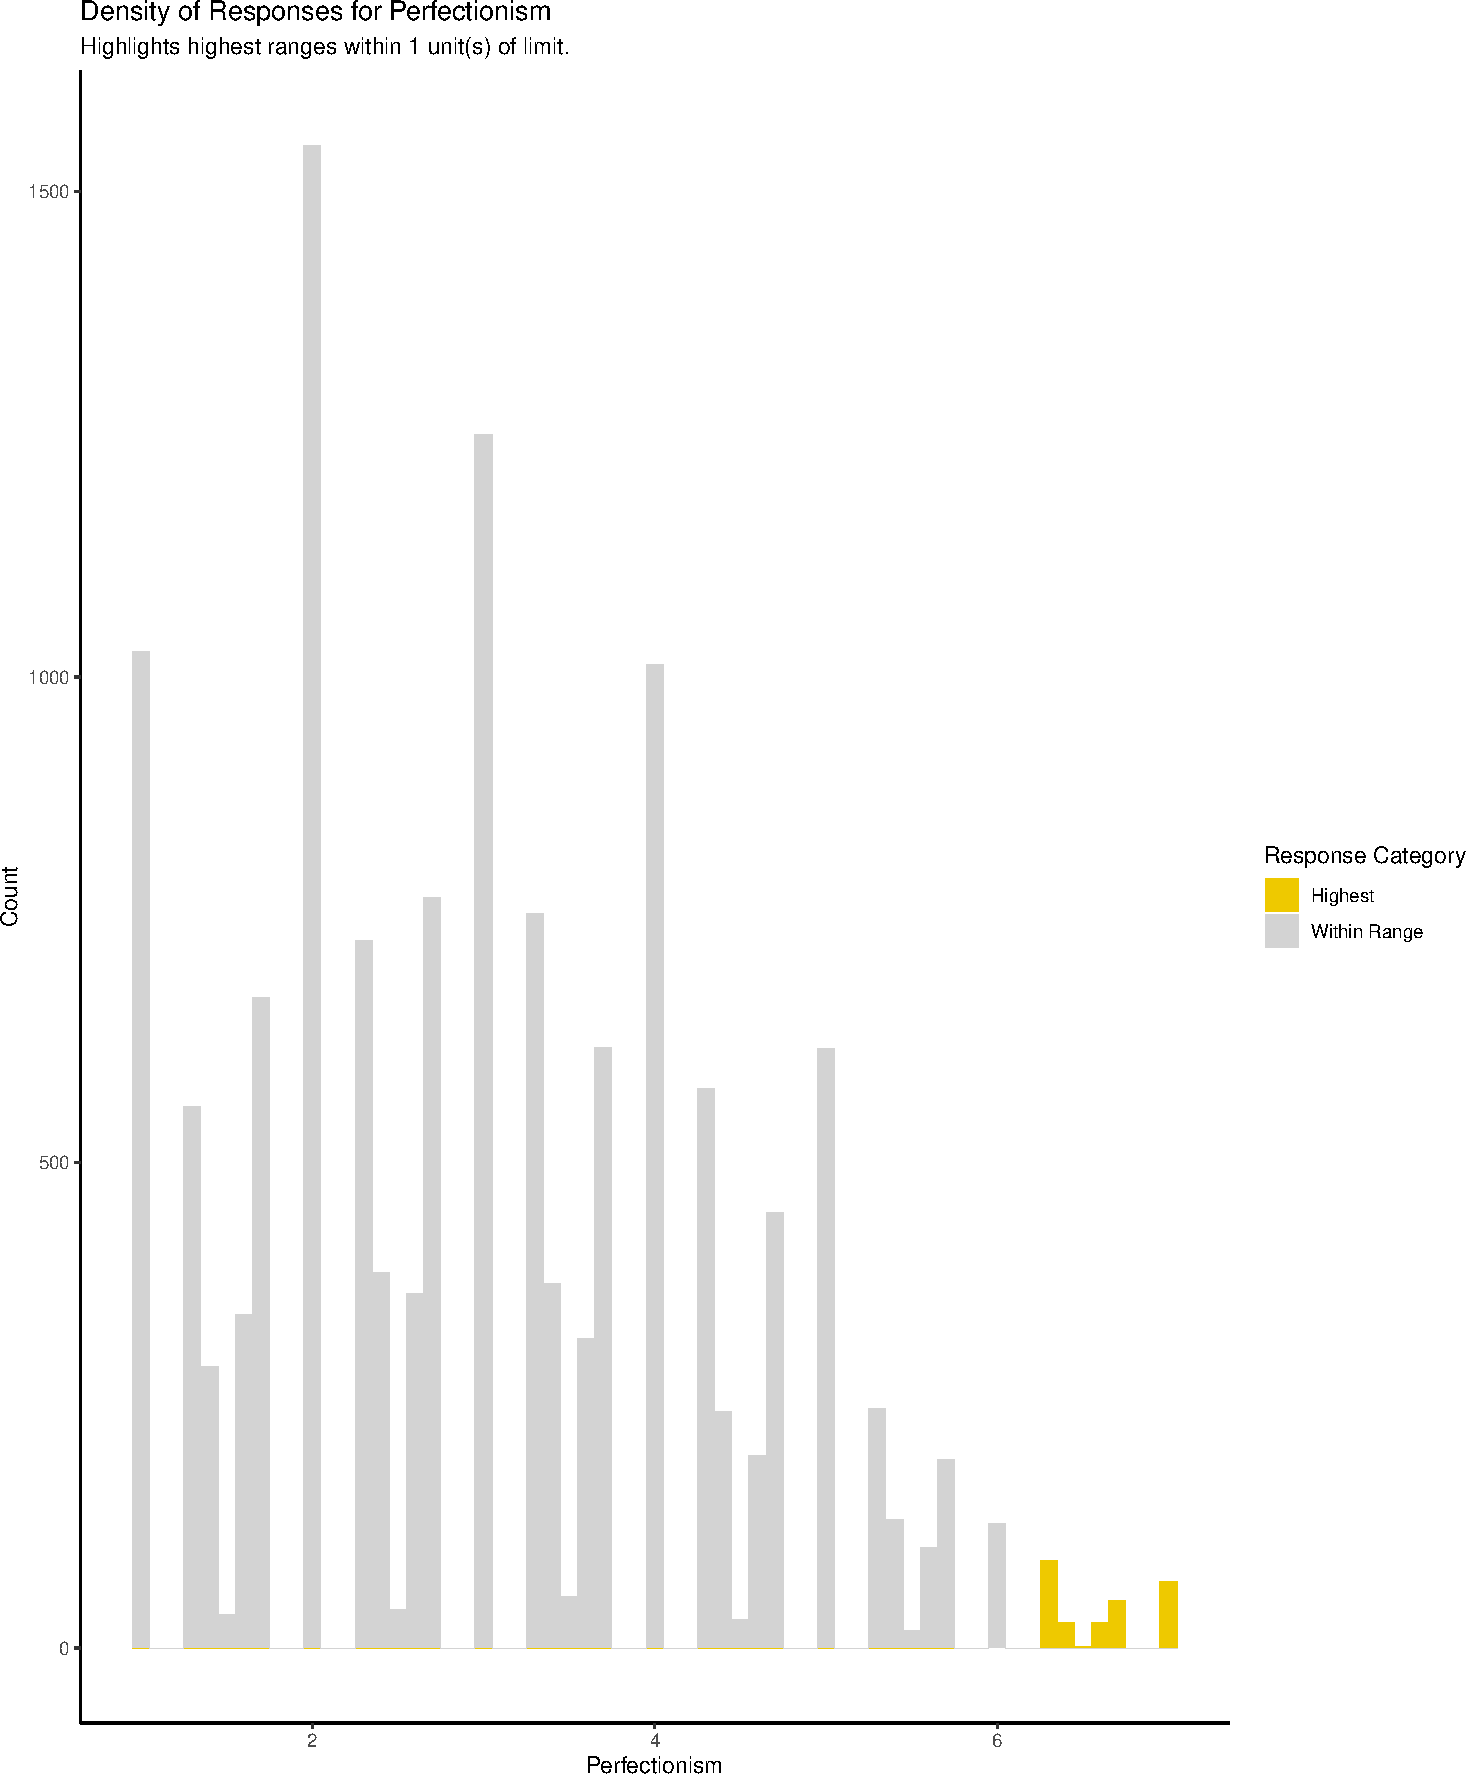
\includegraphics{example-manuscript_files/figure-pdf/fig-hist-1.pdf}

}

\caption{\label{fig-hist}This figure shows a histogram of responses to
religious service frequency in the baseline + 1 wave. Responses above
eight were assigned to eight, and values were rounded to the nearest
whole number. The red dashed line shows the population average. (A)
Responses in the gold bars are shifted to four on the Regular Religious
Service intervention. All those responses in grey (four and above)
remain unchanged. (B) On the zero-intervention, responses in the blue
bars denote those shifted under the zero-intervention treatment.}

\end{figure}%

\newpage{}

\subsubsection{Evidence for Change in the Treatment
Variable}\label{evidence-for-change-in-the-treatment-variable}

Table~\ref{tbl-transition} clarifies the change in the treatment
variable from the baseline wave to the baseline + 1 wave across the
sample. Assessing change in a variable is essential for evaluating the
positivity assumption and recovering evidence for the incident exposure
effect of the treatment variable (\citeproc{ref-danaei2012}{Danaei
\emph{et al.} 2012}; \citeproc{ref-hernan2024WHATIF}{Hernan and Robins
2024}; \citeproc{ref-vanderweele2020}{VanderWeele \emph{et al.} 2020}).
We find that state 4 (weekly attendance) and state 0 present the highest
overall. However, movement between these states reveals they are not
deterministic. States 1, 2, 3, and 5 exhibit more frequent jumps in and
out of these states, suggesting lower stability and/or measurement
error.

\begin{longtable}[]{@{}
  >{\centering\arraybackslash}p{(\columnwidth - 14\tabcolsep) * \real{0.1200}}
  >{\centering\arraybackslash}p{(\columnwidth - 14\tabcolsep) * \real{0.1200}}
  >{\centering\arraybackslash}p{(\columnwidth - 14\tabcolsep) * \real{0.1333}}
  >{\centering\arraybackslash}p{(\columnwidth - 14\tabcolsep) * \real{0.1333}}
  >{\centering\arraybackslash}p{(\columnwidth - 14\tabcolsep) * \real{0.1333}}
  >{\centering\arraybackslash}p{(\columnwidth - 14\tabcolsep) * \real{0.1200}}
  >{\centering\arraybackslash}p{(\columnwidth - 14\tabcolsep) * \real{0.1200}}
  >{\centering\arraybackslash}p{(\columnwidth - 14\tabcolsep) * \real{0.1200}}@{}}

\caption{\label{tbl-transition}This transition matrix captures shifts in
states across across the treatment intervals. Each cell in the matrix
represents the count of individuals transitioning from one state to
another. The rows correspond to the treatment at baseline (From), and
the columns correspond to the state at the following wave (To).
\textbf{Diagonal entries} (in \textbf{bold}) correspond to the number of
individuals who remained in their initial state across both waves.
\textbf{Off-diagonal entries} correspond to the transitions of
individuals from their baseline state to a different state in the
treatment wave. A higher number on the diagonal relative to the
off-diagonal entries in the same row indicates greater stability in a
state. Conversely, higher off-diagonal numbers suggest more frequent
shifts from the baseline state to other states.}

\tabularnewline

\toprule\noalign{}
\begin{minipage}[b]{\linewidth}\centering
From
\end{minipage} & \begin{minipage}[b]{\linewidth}\centering
State 1
\end{minipage} & \begin{minipage}[b]{\linewidth}\centering
State 2
\end{minipage} & \begin{minipage}[b]{\linewidth}\centering
State 3
\end{minipage} & \begin{minipage}[b]{\linewidth}\centering
State 4
\end{minipage} & \begin{minipage}[b]{\linewidth}\centering
State 5
\end{minipage} & \begin{minipage}[b]{\linewidth}\centering
State 6
\end{minipage} & \begin{minipage}[b]{\linewidth}\centering
State 7
\end{minipage} \\
\midrule\noalign{}
\endhead
\bottomrule\noalign{}
\endlastfoot
State 1 & \textbf{893} & 484 & 194 & 40 & 16 & 3 & 2 \\
State 2 & 657 & \textbf{1737} & 904 & 283 & 78 & 9 & 1 \\
State 3 & 237 & 1073 & \textbf{1368} & 768 & 245 & 40 & 5 \\
State 4 & 66 & 335 & 803 & \textbf{1076} & 523 & 108 & 10 \\
State 5 & 24 & 77 & 253 & 531 & \textbf{579} & 223 & 26 \\
State 6 & 7 & 9 & 38 & 106 & 205 & \textbf{216} & 53 \\
State 7 & 2 & 1 & 5 & 8 & 25 & 45 & \textbf{48} \\

\end{longtable}

\newpage{}

\subsection{Results}\label{results}

\subsubsection{Study 1: Causal Effects of Perfectionism on Anxiety and
Depression}\label{study-1-causal-effects-of-perfectionism-on-anxiety-and-depression}

Results for the treatment contrasts between perfectionism and the status
quo on mental health are displayed in Figure~\ref{fig-1_1} and
Table~\ref{tbl-1_1}. These results are measured on the causal difference
scale.

\begin{figure}

\centering{

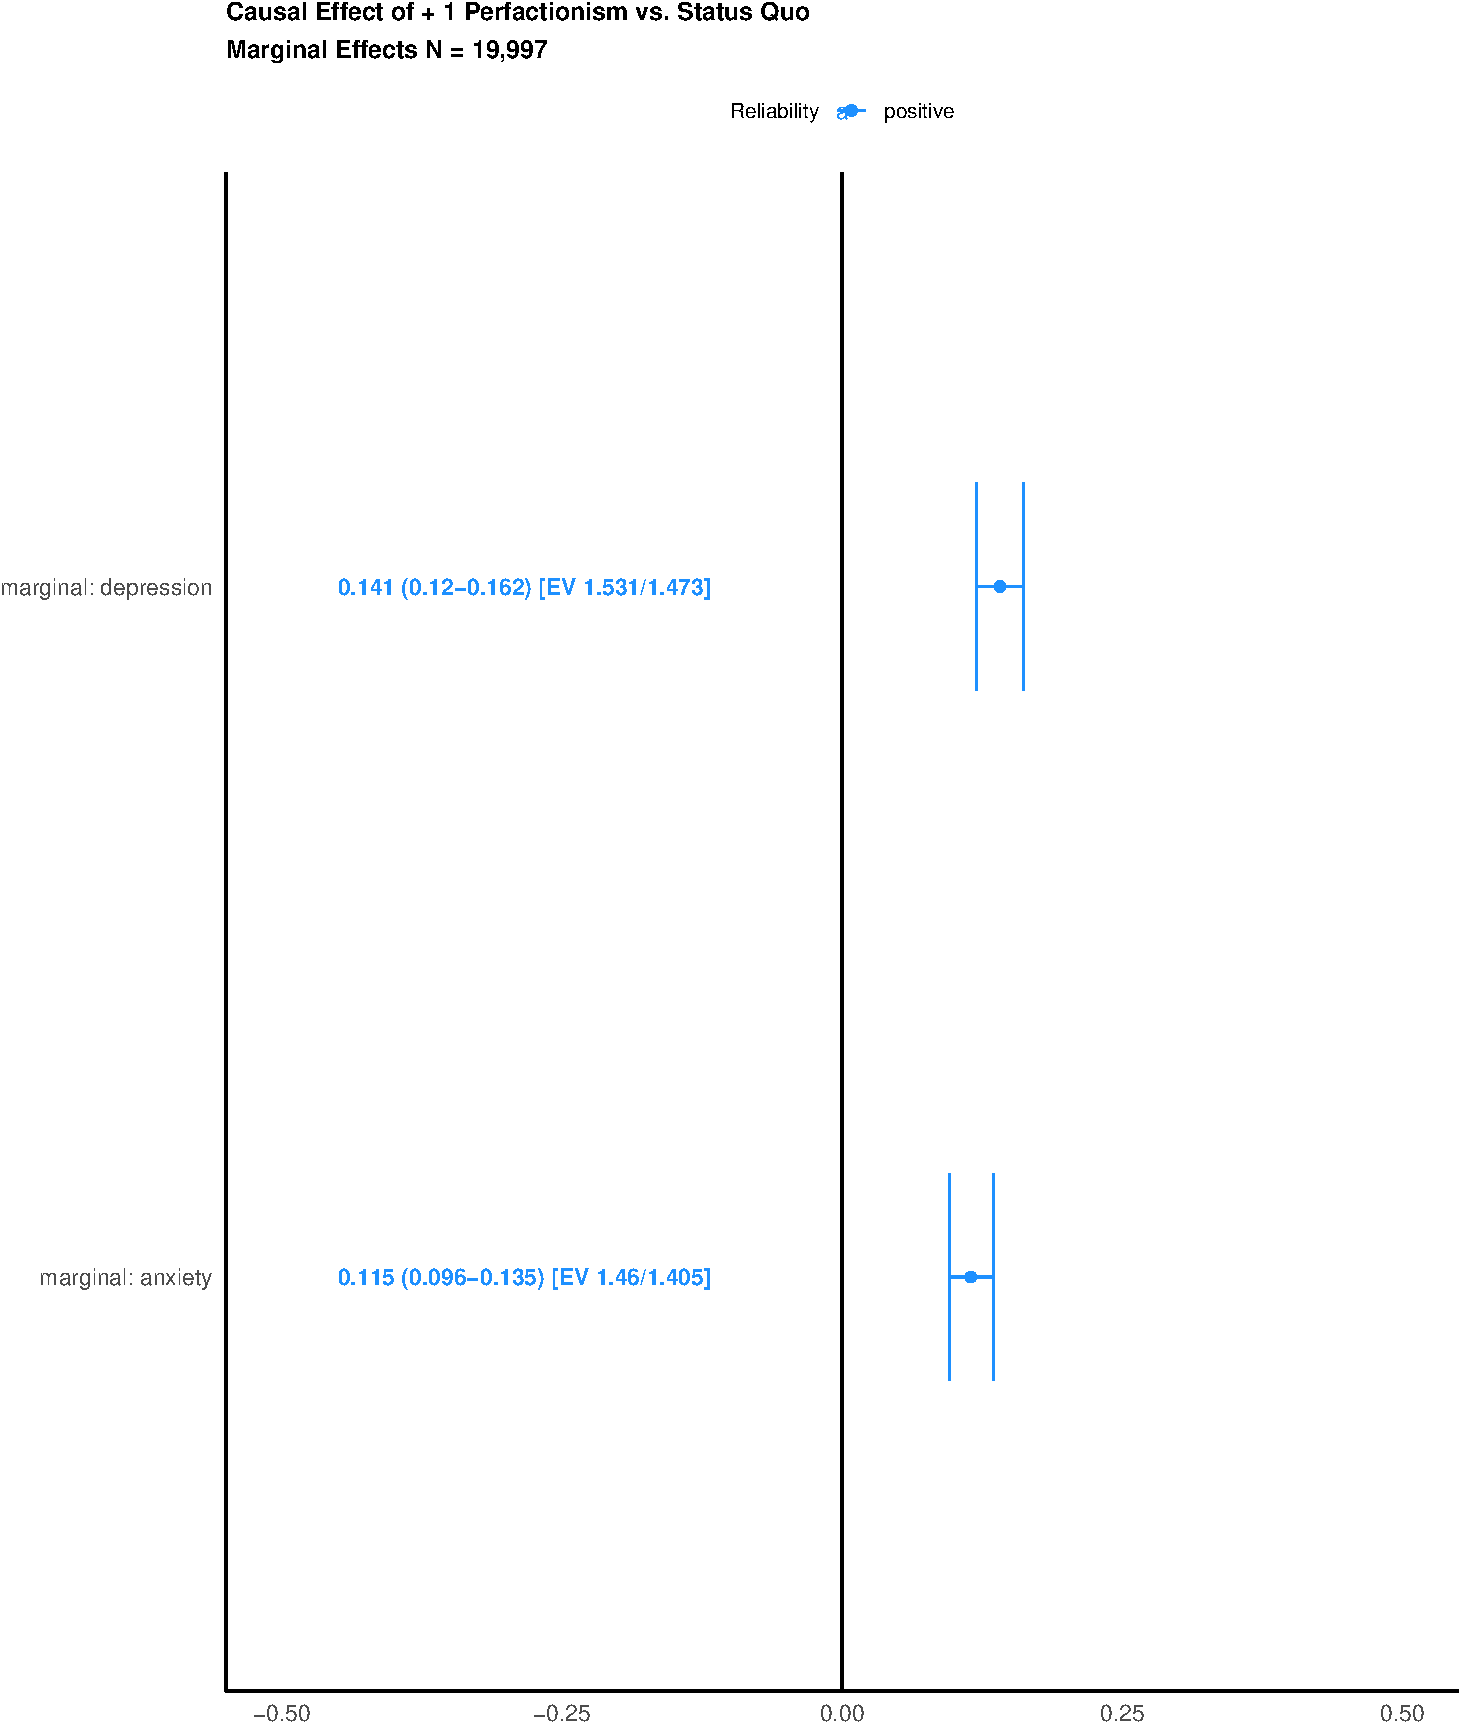
\includegraphics{example-manuscript_files/figure-pdf/fig-1_1-1.pdf}

}

\caption{\label{fig-1_1}This figure reports the results of model
estimates for the causal effects of a one unit increase in perfectionism
vs the status quo depression and anxiety at the end of the study.
Contrasts are expressed in standard deviation units.}

\end{figure}%

\begin{longtable}[]{@{}
  >{\raggedright\arraybackslash}p{(\columnwidth - 10\tabcolsep) * \real{0.3000}}
  >{\raggedleft\arraybackslash}p{(\columnwidth - 10\tabcolsep) * \real{0.2286}}
  >{\raggedleft\arraybackslash}p{(\columnwidth - 10\tabcolsep) * \real{0.0857}}
  >{\raggedleft\arraybackslash}p{(\columnwidth - 10\tabcolsep) * \real{0.1000}}
  >{\raggedleft\arraybackslash}p{(\columnwidth - 10\tabcolsep) * \real{0.1143}}
  >{\raggedleft\arraybackslash}p{(\columnwidth - 10\tabcolsep) * \real{0.1714}}@{}}

\caption{\label{tbl-1_1}This table reports the results of model
estimates for the causal effects of a one unit increase in perfectionism
vs the status quo depression and anxiety at the end of the study.
Contrasts are expressed in standard deviation units.}

\tabularnewline

\toprule\noalign{}
\begin{minipage}[b]{\linewidth}\raggedright
\end{minipage} & \begin{minipage}[b]{\linewidth}\raggedleft
E{[}Y(1){]}-E{[}Y(0){]}
\end{minipage} & \begin{minipage}[b]{\linewidth}\raggedleft
2.5 \%
\end{minipage} & \begin{minipage}[b]{\linewidth}\raggedleft
97.5 \%
\end{minipage} & \begin{minipage}[b]{\linewidth}\raggedleft
E\_Value
\end{minipage} & \begin{minipage}[b]{\linewidth}\raggedleft
E\_Val\_bound
\end{minipage} \\
\midrule\noalign{}
\endhead
\bottomrule\noalign{}
\endlastfoot
marginal: anxiety & 0.115 & 0.096 & 0.135 & 1.460 & 1.405 \\
marginal: depression & 0.141 & 0.120 & 0.162 & 1.531 & 1.473 \\

\end{longtable}

A Longitudinal Modified Treatment Policy (LMTP) calculates the expected
outcome difference between treatment and contrast conditions over a
sequential regime of treatments for a prespecified target population.

For `marginal: depression', the effect estimate is 0.141 {[}0.12,
0.162{]}. The E-value for this estimate is 1.531, with a lower bound of
1.473. At this lower bound, unmeasured confounders would need a minimum
association strength with both the intervention sequence and outcome of
1.473 to negate the observed effect. Weaker confounding would not
overturn it. We infer \textbf{evidence for causality}.

For `marginal: anxiety', the effect estimate is 0.115 {[}0.096,
0.135{]}. The E-value for this estimate is 1.46, with a lower bound of
1.405. At this lower bound, unmeasured confounders would need a minimum
association strength with both the intervention sequence and outcome of
1.405 to negate the observed effect. Weaker confounding would not
overturn it. We infer \textbf{evidence for causality}.

\newpage{}

\paragraph{Subgroup Analysis: Those Born in
NZ}\label{subgroup-analysis-those-born-in-nz}

Figure~\ref{fig-2_1} present results for the treatment contrasts within
the two subgroups, evaluating the effect of a one unit increase in
perfectionism vs the status qu. These results are presented on the
difference scale in standardized units.

Table~\ref{tbl-2_1} presents the results for those born in New Zealand.
Table~\ref{tbl-2_2} presents results for those born overseas.

\begin{figure}

\centering{

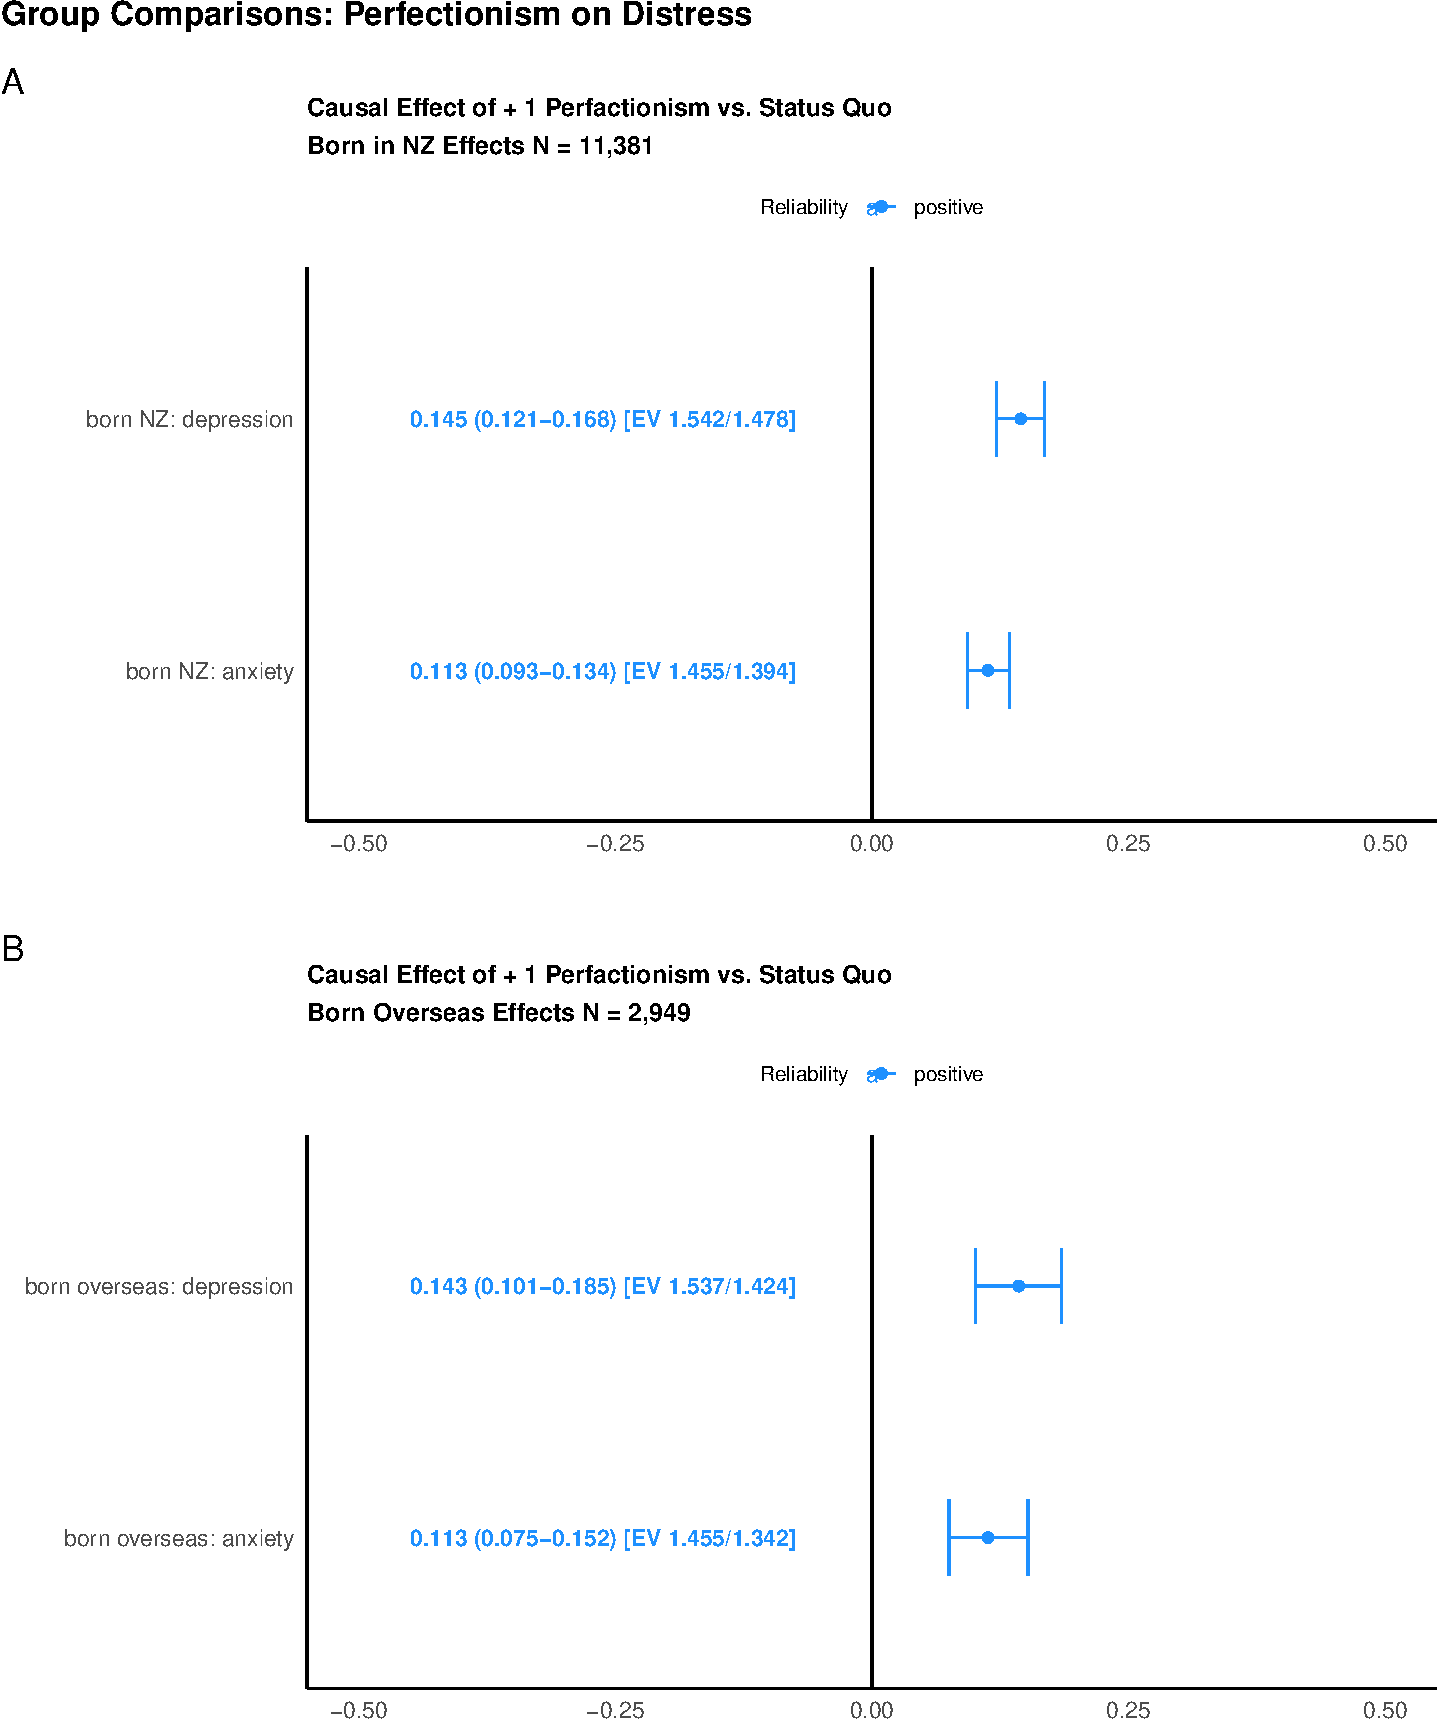
\includegraphics{example-manuscript_files/figure-pdf/fig-2_1-1.pdf}

}

\caption{\label{fig-2_1}This figure reports the results of for each
sub-group analysis for the causal effects of a one unit increase in
perfectionism vs the status quo depression and anxiety at the end of the
study. Contrasts are expressed in standard deviation units.}

\end{figure}%

\begin{longtable}[]{@{}
  >{\raggedright\arraybackslash}p{(\columnwidth - 10\tabcolsep) * \real{0.2899}}
  >{\raggedleft\arraybackslash}p{(\columnwidth - 10\tabcolsep) * \real{0.2319}}
  >{\raggedleft\arraybackslash}p{(\columnwidth - 10\tabcolsep) * \real{0.0870}}
  >{\raggedleft\arraybackslash}p{(\columnwidth - 10\tabcolsep) * \real{0.1014}}
  >{\raggedleft\arraybackslash}p{(\columnwidth - 10\tabcolsep) * \real{0.1159}}
  >{\raggedleft\arraybackslash}p{(\columnwidth - 10\tabcolsep) * \real{0.1739}}@{}}

\caption{\label{tbl-2_1}This table reports the results of model
estimates for in the population of residents born in New Zealand. We
again estimate the causal effects of a one unit increase in
perfectionism vs the status quo depression and anxiety at the end of the
study. Contrasts are expressed in standard deviation units..}

\tabularnewline

\toprule\noalign{}
\begin{minipage}[b]{\linewidth}\raggedright
\end{minipage} & \begin{minipage}[b]{\linewidth}\raggedleft
E{[}Y(1){]}-E{[}Y(0){]}
\end{minipage} & \begin{minipage}[b]{\linewidth}\raggedleft
2.5 \%
\end{minipage} & \begin{minipage}[b]{\linewidth}\raggedleft
97.5 \%
\end{minipage} & \begin{minipage}[b]{\linewidth}\raggedleft
E\_Value
\end{minipage} & \begin{minipage}[b]{\linewidth}\raggedleft
E\_Val\_bound
\end{minipage} \\
\midrule\noalign{}
\endhead
\bottomrule\noalign{}
\endlastfoot
born NZ: anxiety & 0.113 & 0.093 & 0.134 & 1.455 & 1.394 \\
born NZ: depression & 0.145 & 0.121 & 0.168 & 1.542 & 1.478 \\

\end{longtable}

For `born NZ: depression', the effect estimate is 0.145 {[}0.121,
0.168{]}. The E-value for this estimate is 1.542, with a lower bound of
1.478. At this lower bound, unmeasured confounders would need a minimum
association strength with both the intervention sequence and outcome of
1.478 to negate the observed effect. Weaker confounding would not
overturn it. We infer \textbf{evidence for causality}.

For `born NZ: anxiety', the effect estimate is 0.113 {[}0.093, 0.134{]}.
The E-value for this estimate is 1.455, with a lower bound of 1.394. At
this lower bound, unmeasured confounders would need a minimum
association strength with both the intervention sequence and outcome of
1.394 to negate the observed effect. Weaker confounding would not
overturn it. We infer \textbf{evidence for causality}.

\begin{longtable}[]{@{}
  >{\raggedright\arraybackslash}p{(\columnwidth - 10\tabcolsep) * \real{0.3467}}
  >{\raggedleft\arraybackslash}p{(\columnwidth - 10\tabcolsep) * \real{0.2133}}
  >{\raggedleft\arraybackslash}p{(\columnwidth - 10\tabcolsep) * \real{0.0800}}
  >{\raggedleft\arraybackslash}p{(\columnwidth - 10\tabcolsep) * \real{0.0933}}
  >{\raggedleft\arraybackslash}p{(\columnwidth - 10\tabcolsep) * \real{0.1067}}
  >{\raggedleft\arraybackslash}p{(\columnwidth - 10\tabcolsep) * \real{0.1600}}@{}}

\caption{\label{tbl-2_2}This table reports the results of model
estimates for in the population of residents not born in New Zealand
(born overseas). We again estimate the causal effects of a one unit
increase in perfectionism vs the status quo depression and anxiety at
the end of the study. Contrasts are expressed in standard deviation
units.}

\tabularnewline

\toprule\noalign{}
\begin{minipage}[b]{\linewidth}\raggedright
\end{minipage} & \begin{minipage}[b]{\linewidth}\raggedleft
E{[}Y(1){]}-E{[}Y(0){]}
\end{minipage} & \begin{minipage}[b]{\linewidth}\raggedleft
2.5 \%
\end{minipage} & \begin{minipage}[b]{\linewidth}\raggedleft
97.5 \%
\end{minipage} & \begin{minipage}[b]{\linewidth}\raggedleft
E\_Value
\end{minipage} & \begin{minipage}[b]{\linewidth}\raggedleft
E\_Val\_bound
\end{minipage} \\
\midrule\noalign{}
\endhead
\bottomrule\noalign{}
\endlastfoot
born overseas: anxiety & 0.113 & 0.075 & 0.152 & 1.455 & 1.342 \\
born overseas: depression & 0.143 & 0.101 & 0.185 & 1.537 & 1.424 \\

\end{longtable}

For `born overseas: depression', the effect estimate is 0.143 {[}0.101,
0.185{]}. The E-value for this estimate is 1.537, with a lower bound of
1.424. At this lower bound, unmeasured confounders would need a minimum
association strength with both the intervention sequence and outcome of
1.424 to negate the observed effect. Weaker confounding would not
overturn it. We infer \textbf{evidence for causality}.

For `born overseas: anxiety', the effect estimate is 0.113 {[}0.075,
0.152{]}. The E-value for this estimate is 1.455, with a lower bound of
1.342. At this lower bound, unmeasured confounders would need a minimum
association strength with both the intervention sequence and outcome of
1.342 to negate the observed effect. Weaker confounding would not
overturn it. We infer \textbf{evidence for causality}.

\subsection{Findings}\label{findings}

Comparing the difference in the mean outcomes between to the two groups
for anxiety: The difference in means is 2e-04 with a standard error of
0.0223 and a 95\% CI of {[}-0.0436, 0.0439{]}.. We therefore do not
detect a reliable difference between those born in New Zealand and those
born elsewhere.

Comparing the difference in the mean outcomes between to the two groups
for depression: The difference in means is 2e-04 with a standard error
of 0.0223 and a 95\% CI of {[}-0.0436, 0.0439{]}.. We therefore do not
detect a reliable difference between those born in New Zealand and those
born elsewhere.

\newpage{}

\subsubsection{Additional Study: Comparison of Causal Inference Results
with Cross-Sectional
Regressions}\label{additional-study-comparison-of-causal-inference-results-with-cross-sectional-regressions}

To better evaluate the contributions of our methodology to current
practice, we conducted a series of cross-sectional analyses using the
baseline wave data. We quantified the statistical associations between
religious service attendance and our focal prosocial outcomes. We
included all regression covariates from the causal models (including
sample weights) for each analysis, obviously omitting the outcome
measured at baseline, i.e.~the response variable.

\textbf{Cross-sectional anxiety result}: the change in expected
kessler-6 anxiety for a one-unit increase in perfectionism is b = 0.31;
(95\% CI 0.30, 0.32). This result is 2.65 per cent greater than the
effect estimated from the `+1 vs.~status quo' causal contrast (0.115),
indicating an \textbf{overstatement in the cross-sectional regression
model.}

\textbf{Cross-sectional depression result}: the change in expected
kessler-6 depression for a one-unit increase in perfectionism is b =
0.34; (95\% CI 0.33, 0.35). This result is 2.43 per cent greater than
the effect estimated from the `+1 vs.~status quo' causal contrast
(0.141), indicating an \textbf{overstatement in the cross-sectional
regression model.}

These findings underscore that the results of cross-sectional
regressions, although suggestive, can considerably diverge from those
obtained from the causal analysis of panel data.

\newpage{}

\subsection{Discussion}\label{discussion}

\subsubsection{Considerations}\label{considerations}

First, as stated above, our causal inferences turn on three assumptions,
which are worth revisiting:

(i). \textbf{Unmeasured confounding}: although we employ robust methods
for causal inference, our results depend on the effectiveness of our
strategy to control for confounding. Our sensitivity analyses address
the potential impacts of unmeasured confounders. Nevertheless, the
presence and influence of such confounders are uncertain and
unverifiable from our data.

(ii). \textbf{Causal consistency}: the observed outcomes must correspond
to the counterfactual treatments contrasted. Although ``religious
service attendance'' may appear conditionally independent of the
outcomes given baseline covariates, interpreting these interventions
remains challenging. ``Religious service attendance'' varies widely,
encompassing everything from informal gatherings at homes to formal
services in cathedrals across New Zealand's religious diversity. This
type of ``treatment'' does not mirror a straightforward medical
intervention like a vaccine. The heterogeneity of ``religious service''
limits the clarity of our results, an issue no amount of data or
analysis can resolve because ``religious service'' reflects a broad
spectrum of community activities.

(iii). \textbf{Positivity}: we have confirmed that religious service
attendance varies within our sample and have used semi-parametric models
with ensemble learning and cross-validation to prevent data
over-extrapolation and model over-fitting. Conceptually, it is crucial
for valid causal inference that every potential level of ``treatment''
to religious services is realistically possible (refer to discussion in
VanderWeele (\citeproc{ref-vanderweele2017causaleffectsService}{2017})).
Although there are instances realised in our data of secular individuals
initiating religious service and frequent attendees stopping (refer to
Table~\ref{tbl-transition}), it might stretch credulity too far to
imagine that such changes are possible for everyone.

Second, our study confronts the spectre of \textbf{measurement error}:
both direct and correlated measurement errors can introduce biases,
either by implying effects where none exist or by attenuating true
effects (\citeproc{ref-vanderweele2012MEASUREMENT}{VanderWeele and
Hernán 2012}). Importantly, evaluating prosociality using multiple
measures while also controlling for these measures and the treatment at
baseline helps to mitigate measurement error concerns. Nevertheless,
unknown combinations of measurement error might nevertheless bias our
results. The outcomes and estimates we report here are best-considered
approximations.

Third, we do not examine \textbf{treatment effect heterogeneity}:
identifying which subgroups experience the strongest responses remains a
task for future research. Such investigations are crucial for making
informed policy decisions and tailoring advice relevant to those
subgroups of the population who might benefit most. Perhaps the most
obvious stratum is religious affiliates
(\citeproc{ref-vanderweele2017causaleffectsService}{VanderWeele 2017}).

Fourth, the \textbf{transportability of our findings remains unclear}:
New Zealand is our target population. Our findings generalise to this
population. However, the transportability of our findings to other
settings---whether our results generalise beyond our targeted New
Zealand population---remains an open question, a matter for future
investigations.

\subsubsection{Observations and
Recommendations}\label{observations-and-recommendations}

\newpage{}

\subsubsection{Ethics}\label{ethics}

\{\textbf{authors blinded}\}

\subsubsection{Data Availability}\label{data-availability}

\{\textbf{authors blinded}\}

\subsubsection{Acknowledgements}\label{acknowledgements}

\{\textbf{authors blinded}\}

\subsubsection{Author Statement}\label{author-statement}

\{\textbf{authors blinded}\}

\newpage{}

\subsection{Appendix A: Measures}\label{appendix-measures}

\paragraph{Age (waves: 1-15)}\label{age-waves-1-15}

We asked participants' ages in an open-ended question (``What is your
age?'' or ``What is your date of birth?'').

\paragraph{Born in New Zealand}\label{born-in-new-zealand}

\paragraph{Charitable Donations (Study 1
outcome)}\label{charitable-donations-study-1-outcome}

Using one item from Hoverd and Sibley
(\citeproc{ref-hoverd_religious_2010}{2010}), we asked participants,
``How much money have you donated to charity in the last year?''.

\paragraph{Charitable Volunteering (Study 1
outcome)}\label{charitable-volunteering-study-1-outcome}

We measured hours of volunteering using one item from Sibley \emph{et
al.} (\citeproc{ref-sibley2011}{2011}): ``Hours spent \ldots{}
voluntary/charitable work.''

\paragraph{Children Number (waves: 1-3,
4-15)}\label{children-number-waves-1-3-4-15}

We measured the number of children using one item from Bulbulia \emph{et
al.} (\citeproc{ref-Bulbulia_2015}{2015}). We asked participants, ``How
many children have you given birth to, fathered, or adopted. How many
children have you given birth to, fathered, or adopted?'' or ``How many
children have you given birth to, fathered, or adopted. How many
children have you given birth to, fathered, and/or parented?'' (waves:
12-15).

\paragraph{Disability}\label{disability}

We assessed disability with a one-item indicator adapted from Verbrugge
(\citeproc{ref-verbrugge1997}{1997}). It asks, ``Do you have a health
condition or disability that limits you and that has lasted for 6+
months?'' (1 = Yes, 0 = No).

\paragraph{Education Attainment (waves: 1,
4-15)}\label{education-attainment-waves-1-4-15}

We asked participants, ``What is your highest level of qualification?''.
We coded participants' highest finished degree according to the New
Zealand Qualifications Authority. Ordinal-Rank 0-10 NZREG codes (with
overseas school quals coded as Level 3, and all other ancillary
categories coded as missing)
See:https://www.nzqa.govt.nz/assets/Studying-in-NZ/New-Zealand-Qualification-Framework/requirements-nzqf.pdf

\paragraph{Employment (waves: 1-3,
4-11)}\label{employment-waves-1-3-4-11}

We asked participants, ``Are you currently employed? (This includes
self-employed or casual work)''.

\paragraph{Ethnicity}\label{ethnicity}

Based on the New Zealand Census, we asked participants, ``Which ethnic
group(s) do you belong to?''. The responses were: (1) New Zealand
European; (2) Māori; (3) Samoan; (4) Cook Island Māori; (5) Tongan; (6)
Niuean; (7) Chinese; (8) Indian; (9) Other such as DUTCH, JAPANESE,
TOKELAUAN. Please state:. We coded their answers into four groups:
Maori, Pacific, Asian, and Euro (except for Time 3, which used an
open-ended measure).

\paragraph{Fatigue}\label{fatigue}

We assessed subjective fatigue by asking participants, ``During the last
30 days, how often did \ldots{} you feel exhausted?'' Responses were
collected on an ordinal scale (0 = None of The Time, 1 = A little of The
Time, 2 = Some of The Time, 3 = Most of The Time, 4 = All of The Time).

\paragraph{Honesty-Humility-Modesty Facet (waves:
10-14)}\label{honesty-humility-modesty-facet-waves-10-14}

Participants indicated the extent to which they agree with the following
four statements from Campbell \emph{et al.}
(\citeproc{ref-campbell2004}{2004}) , and Sibley \emph{et al.}
(\citeproc{ref-sibley2011}{2011}) (1 = Strongly Disagree to 7 = Strongly
Agree)

\begin{verbatim}
i.  I want people to know that I am an important person of high status, (Waves: 1, 10-14)
ii. I am an ordinary person who is no better than others.
iii. I wouldn't want people to treat me as though I were superior to them.
iv. I think that I am entitled to more respect than the average person is.
\end{verbatim}

\paragraph{Hours of Childcare}\label{hours-of-childcare}

We measured hours of exercising using one item from Sibley \emph{et al.}
(\citeproc{ref-sibley2011}{2011}): 'Hours spent \ldots{} looking after
children.''

To stabilise this indicator, we took the natural log of the response +
1.

\paragraph{Hours of Housework}\label{hours-of-housework}

We measured hours of exercising using one item from Sibley \emph{et al.}
(\citeproc{ref-sibley2011}{2011}): ``Hours spent \ldots{}
housework/cooking''

To stabilise this indicator, we took the natural log of the response +
1.

\paragraph{Hours of Exercise}\label{hours-of-exercise}

We measured hours of exercising using one item from Sibley \emph{et al.}
(\citeproc{ref-sibley2011}{2011}): ``Hours spent \ldots{}
exercising/physical activity''

To stabilise this indicator, we took the natural log of the response +
1.

\paragraph{Hours of Childcare}\label{hours-of-childcare-1}

We measured hours of exercising using one item from Sibley \emph{et al.}
(\citeproc{ref-sibley2011}{2011}): 'Hours spent \ldots{} looking after
children.''

To stabilise this indicator, we took the natural log of the response +
1.

\paragraph{Hours of Exercise}\label{hours-of-exercise-1}

We measured hours of exercising using one item from Sibley \emph{et al.}
(\citeproc{ref-sibley2011}{2011}): ``Hours spent \ldots{}
exercising/physical activity''

To stabilise this indicator, we took the natural log of the response +
1.

\paragraph{Hours of Housework}\label{hours-of-housework-1}

We measured hours of exercising using one item from Sibley \emph{et al.}
(\citeproc{ref-sibley2011}{2011}): ``Hours spent \ldots{}
housework/cooking''

To stabilise this indicator, we took the natural log of the response +
1.

\paragraph{Hours of Sleep}\label{hours-of-sleep}

Participants were asked, ``During the past month, on average, how many
hours of \emph{actual sleep} did you get per night?''.

\paragraph{Hours of Work}\label{hours-of-work}

We measured work hours using one item from Sibley \emph{et al.}
(\citeproc{ref-sibley2011}{2011}): ``Hours spent \ldots{} working in
paid employment.''

To stabilise this indicator, we took the natural log of the response +
1.

\paragraph{Income (waves: 1-3, 4-15)}\label{income-waves-1-3-4-15}

Participants were asked, ``Please estimate your total household income
(before tax) for the year XXXX''. To stabilise this indicator, we first
took the natural log of the response + 1, and then centred and
standardised the log-transformed indicator.

\paragraph{Kessler-6: Psychological Distress (waves:
2-3,4-15)}\label{kessler-6-psychological-distress-waves-2-34-15}

We measured psychological distress using the Kessler-6 scale
(kessler2002?), which exhibits strong diagnostic concordance for
moderate and severe psychological distress in large, crosscultural
samples (kessler2010?; prochaska2012?). Participants rated during the
past 30 days, how often did\ldots{} (1) ``\ldots{} you feel hopeless'';
(2) ``\ldots{} you feel so depressed that nothing could cheer you up'';
(3) ``\ldots{} you feel restless or fidgety''; (4)``\ldots{} you feel
that everything was an effort''; (5) ``\ldots{} you feel worthless'';
(6) '' you feel nervous?'' Ordinal response alternatives for the
Kessler-6 are: ``None of the time''; ``A little of the time''; ``Some of
the time''; ``Most of the time''; ``All of the time.''

\paragraph{Male Gender (waves: 1-15)}\label{male-gender-waves-1-15}

We asked participants' gender in an open-ended question: ``what is your
gender?'' or ``Are you male or female?'' (waves: 1-5). Female was coded
as 0, Male as 1, and gender diverse coded as 3
(\citeproc{ref-fraser_coding_2020}{Fraser \emph{et al.} 2020}). (or 0.5
= neither female nor male)

Here, we coded all those who responded as Male as 1, and those who did
not as 0.

\paragraph{Mini-IPIP 6 (waves:
1-3,4-15)}\label{mini-ipip-6-waves-1-34-15}

We measured participants' personalities with the Mini International
Personality Item Pool 6 (Mini-IPIP6) (\citeproc{ref-sibley2011}{Sibley
\emph{et al.} 2011}), which consists of six dimensions and each
dimension is measured with four items:

\begin{enumerate}
\def\labelenumi{\arabic{enumi}.}
\item
  agreeableness,

  \begin{enumerate}
  \def\labelenumii{\roman{enumii}.}
  \tightlist
  \item
    I sympathize with others' feelings.
  \item
    I am not interested in other people's problems. (r)
  \item
    I feel others' emotions.
  \item
    I am not really interested in others. (r)
  \end{enumerate}
\item
  conscientiousness,

  \begin{enumerate}
  \def\labelenumii{\roman{enumii}.}
  \tightlist
  \item
    I get chores done right away.
  \item
    I like order.
  \item
    I make a mess of things. (r)
  \item
    I often forget to put things back in their proper place. (r)
  \end{enumerate}
\item
  extraversion,

  \begin{enumerate}
  \def\labelenumii{\roman{enumii}.}
  \tightlist
  \item
    I am the life of the party.
  \item
    I don't talk a lot. (r)
  \item
    I keep in the background. (r)
  \item
    I talk to a lot of different people at parties.
  \end{enumerate}
\item
  honesty-humility,

  \begin{enumerate}
  \def\labelenumii{\roman{enumii}.}
  \tightlist
  \item
    I feel entitled to more of everything. (r)
  \item
    I deserve more things in life. (r)
  \item
    I would like to be seen driving around in a very expensive car. (r)
  \item
    I would get a lot of pleasure from owning expensive luxury goods.
    (r)
  \end{enumerate}
\item
  neuroticism, and

  \begin{enumerate}
  \def\labelenumii{\roman{enumii}.}
  \tightlist
  \item
    I have frequent mood swings.
  \item
    I am relaxed most of the time. (r)
  \item
    I get upset easily.
  \item
    I seldom feel blue. (r)
  \end{enumerate}
\item
  openness to experience

  \begin{enumerate}
  \def\labelenumii{\roman{enumii}.}
  \tightlist
  \item
    I have a vivid imagination.
  \item
    I have difficulty understanding abstract ideas. (r)
  \item
    I do not have a good imagination. (r)
  \item
    I am not interested in abstract ideas. (r)
  \end{enumerate}
\end{enumerate}

Each dimension was assessed with four items and participants rated the
accuracy of each item as it applies to them from 1 (Very Inaccurate) to
7 (Very Accurate). Items marked with (r) are reverse coded.

\paragraph{NZ-Born (waves: 1-2,4-15)}\label{nz-born-waves-1-24-15}

We asked participants, ``Which country were you born in?'' or ``Where
were you born? (please be specific, e.g., which town/city?)'' (waves:
6-15).

\paragraph{NZ Deprivation Index (waves:
1-15)}\label{nz-deprivation-index-waves-1-15}

We used the NZ Deprivation Index to assign each participant a score
based on where they live (\citeproc{ref-atkinson2019}{Atkinson \emph{et
al.} 2019}). This score combines data such as income, home ownership,
employment, qualifications, family structure, housing, and access to
transport and communication for an area into one deprivation score.

\paragraph{NZSEI Occupational Prestige and Status (waves:
8-15)}\label{nzsei-occupational-prestige-and-status-waves-8-15}

We assessed occupational prestige and status using the New Zealand
Socio-economic Index 13 (NZSEI-13) (\citeproc{ref-fahy2017a}{Fahy
\emph{et al.} 2017a}). This index uses the income, age, and education of
a reference group, in this case the 2013 New Zealand census, to
calculate a score for each occupational group. Scores range from 10
(Lowest) to 90 (Highest). This list of index scores for occupational
groups was used to assign each participant an NZSEI-13 score based on
their occupation.

We assessed occupational prestige and status using the New Zealand
Socio-economic Index 13 (NZSEI-13) (\citeproc{ref-fahy2017}{Fahy
\emph{et al.} 2017b}). This index uses the income, age, and education of
a reference group, in this case, the 2013 New Zealand census, to
calculate a score for each occupational group. Scores range from 10
(Lowest) to 90 (Highest). This list of index scores for occupational
groups was used to assign each participant an NZSEI-13 score based on
their occupation.

\paragraph{Opt-in}\label{opt-in}

The New Zealand Attitudes and Values Study allows opt-ins to the study.
Because the opt-in population may differ from those sampled randomly
from the New Zealand electoral roll; although the opt-in rate is low, we
include an indicator (yes/no) for this variable.

\paragraph{Partner (No/Yes)}\label{partner-noyes}

``What is your relationship status?'' (e.g., single, married, de-facto,
civil union, widowed, living together, etc.)

\paragraph{Politically Conservative}\label{politically-conservative}

We measured participants' political conservative orientation using a
single item adapted from Jost (\citeproc{ref-jost_end_2006-1}{2006}).

``Please rate how politically liberal versus conservative you see
yourself as being.''

(1 = Extremely Liberal to 7 = Extremely Conservative)

\subparagraph{Religious Service
Attendance}\label{religious-service-attendance}

If participants answered \emph{yes} to ``Do you identify with a religion
and/or spiritual group?'' we measured their frequency of church
attendence using one item from Sibley and Bulbulia
(\citeproc{ref-sibley2012}{2012}): ``how many times did you attend a
church or place of worship in the last month?''. Those participants who
were not religious were imputed a score of ``0''.

\paragraph{Rural/Urban Codes}\label{ruralurban-codes}

Participants residence locations were coded according to a five-level
ordinal categorisation ranging from ``Urban'' to Rural, see Sibley
(\citeproc{ref-sibley2021}{2021}).

\paragraph{Short-Form Health}\label{short-form-health}

Participants' subjective health was measured using one item (``Do you
have a health condition or disability that limits you, and that has
lasted for 6+ months?''; 1 = Yes, 0 = No) adapted from Verbrugge
(\citeproc{ref-verbrugge1997}{1997}).

\paragraph{Sample Origin}\label{sample-origin}

Wave enrolled in NZAVS, see Sibley (\citeproc{ref-sibley2021}{2021}).

\paragraph{Support received: money (waves 10-12) (Study 4
outcomes)}\label{support-received-money-waves-10-12-study-4-outcomes}

The NZAVS has a `revealed' measure of received help and support measured
in hours of support in the previous week. The items are:

\emph{Please estimate how much help you have received from the following
sources in the last week?}

\begin{itemize}
\tightlist
\item
  \emph{family\ldots MONEY (hours)}
\item
  \emph{friends\ldots MONEY (hours)}
\item
  \emph{members of my community\ldots MONEY (hours)}
\end{itemize}

Because this measure is highly variable, we convert responses to binary
indicators: \emph{0 = none/1 any}

\paragraph{Support received: time (waves 10-13) (Study 3
outcomes)}\label{support-received-time-waves-10-13-study-3-outcomes}

\emph{Please estimate how much help you have received from the following
sources in the last week.}

\begin{itemize}
\tightlist
\item
  \emph{family\ldots TIME (hours)}
\item
  \emph{friends\ldots TIME (hours)}
\item
  \emph{members of my community\ldots TIME (hours)}
\end{itemize}

Because this measure is highly variable, we convert responses to binary
indicators: \emph{0 = none/1 any}

\paragraph{Total Siblings}\label{total-siblings}

Participants were asked the following questions related to sibling
counts:

\begin{itemize}
\tightlist
\item
  Were you the 1st born, 2nd born, or 3rd born, etc, child of your
  mother?
\item
  Do you have siblings?
\item
  How many older sisters do you have?
\item
  How many younger sisters do you have?
\item
  How many older brothers do you have?
\item
  How many younger brothers do you have?
\end{itemize}

A single score was obtained from sibling counts by summing responses to
the ``How many\ldots{}'' items. From these scores, an ordered factor was
created ranging from 0 to 7, where participants with more than 7
siblings were grouped into the highest category.

\newpage{}

\subsection{Appendix B. Baseline Demographic
Statistics}\label{appendix-demographics}

\begin{longtable}[]{@{}ll@{}}

\caption{\label{tbl-table-demography}Baseline demographic statistics}

\tabularnewline

\toprule\noalign{}
\textbf{Exposure + Demographic Variables} & \textbf{N = 19,997} \\
\midrule\noalign{}
\endhead
\bottomrule\noalign{}
\endlastfoot
\textbf{Age} & NA \\
Mean (SD) & 49 (14) \\
Range & 18, 98 \\
IQR & 39, 60 \\
\textbf{Male} & 7,425 (37\%) \\
\textbf{Edu} & NA \\
Mean (SD) & 5.29 (2.72) \\
Range & 0.00, 10.00 \\
IQR & 3.00, 7.00 \\
Unknown & 510 \\
\textbf{Eth Cat} & NA \\
euro & 15,850 (80\%) \\
maori & 2,280 (12\%) \\
pacific & 498 (2.5\%) \\
asian & 1,107 (5.6\%) \\
Unknown & 262 \\
\textbf{Partner} & 14,501 (75\%) \\
Unknown & 649 \\
\textbf{Employed} & 15,884 (80\%) \\
Unknown & 39 \\
\textbf{Born Nz} & 15,436 (78\%) \\
Unknown & 232 \\
\textbf{Neighbourhood Community} & NA \\
Mean (SD) & 4.20 (1.67) \\
Range & 1.00, 7.00 \\
IQR & 2.99, 5.95 \\
Unknown & 113 \\
\textbf{Household Inc log} & NA \\
Mean (SD) & 11.39 (0.76) \\
Range & 0.69, 14.40 \\
IQR & 11.00, 11.92 \\
Unknown & 1,529 \\
\textbf{Parent} & 14,037 (71\%) \\
Unknown & 156 \\
\textbf{Religion Religious} & 7,148 (36\%) \\
Unknown & 301 \\
\textbf{Urban} & 12,291 (62\%) \\
Unknown & 129 \\

\end{longtable}

Table~\ref{tbl-table-demography} baseline demographic statistics for
couples who met inclusion criteria.

\newpage{}

\subsection{Appendix C: Treatment Statistics}\label{appendix-exposures}

\begin{longtable}[]{@{}
  >{\raggedright\arraybackslash}p{(\columnwidth - 4\tabcolsep) * \real{0.4247}}
  >{\raggedright\arraybackslash}p{(\columnwidth - 4\tabcolsep) * \real{0.2877}}
  >{\raggedright\arraybackslash}p{(\columnwidth - 4\tabcolsep) * \real{0.2877}}@{}}

\caption{\label{tbl-table-exposures-code}Exposures at baseline and
baseline + 1 (treatment) wave}

\tabularnewline

\toprule\noalign{}
\begin{minipage}[b]{\linewidth}\raggedright
\textbf{Exposure Variables by Wave}
\end{minipage} & \begin{minipage}[b]{\linewidth}\raggedright
\textbf{2018}, N = 19,997
\end{minipage} & \begin{minipage}[b]{\linewidth}\raggedright
\textbf{2019}, N = 19,997
\end{minipage} \\
\midrule\noalign{}
\endhead
\bottomrule\noalign{}
\endlastfoot
\textbf{Perfectionism} & 3.02 (2.03, 4.04) & 2.99 (2.00, 4.02) \\
Unknown & 0 & 5,558 \\

\end{longtable}

tbl-table-exposures-code presents baseline (NZAVS time 10) and exposure
wave (NZAVS time 11) statistics for the exposure variable: perfectionism
(range 1-7).

\subsubsection{Imbalance of Confounding Covariates
Treatments}\label{imbalance-of-confounding-covariates-treatments}

Figure~\ref{fig-match_1} shows imbalance of covariates on the treatment
at the treatment wave. The variable on which there is strongest
imbalance is the baseline measure of religious service attendance. It is
important to adjust for this measure both for confounding control and to
better estimate an incident exposure effect for the religious service at
the treatment wave (in contrast to merely estimating a prevalence
effect). See VanderWeele \emph{et al.}
(\citeproc{ref-vanderweele2020}{2020}).

\begin{figure}

\centering{

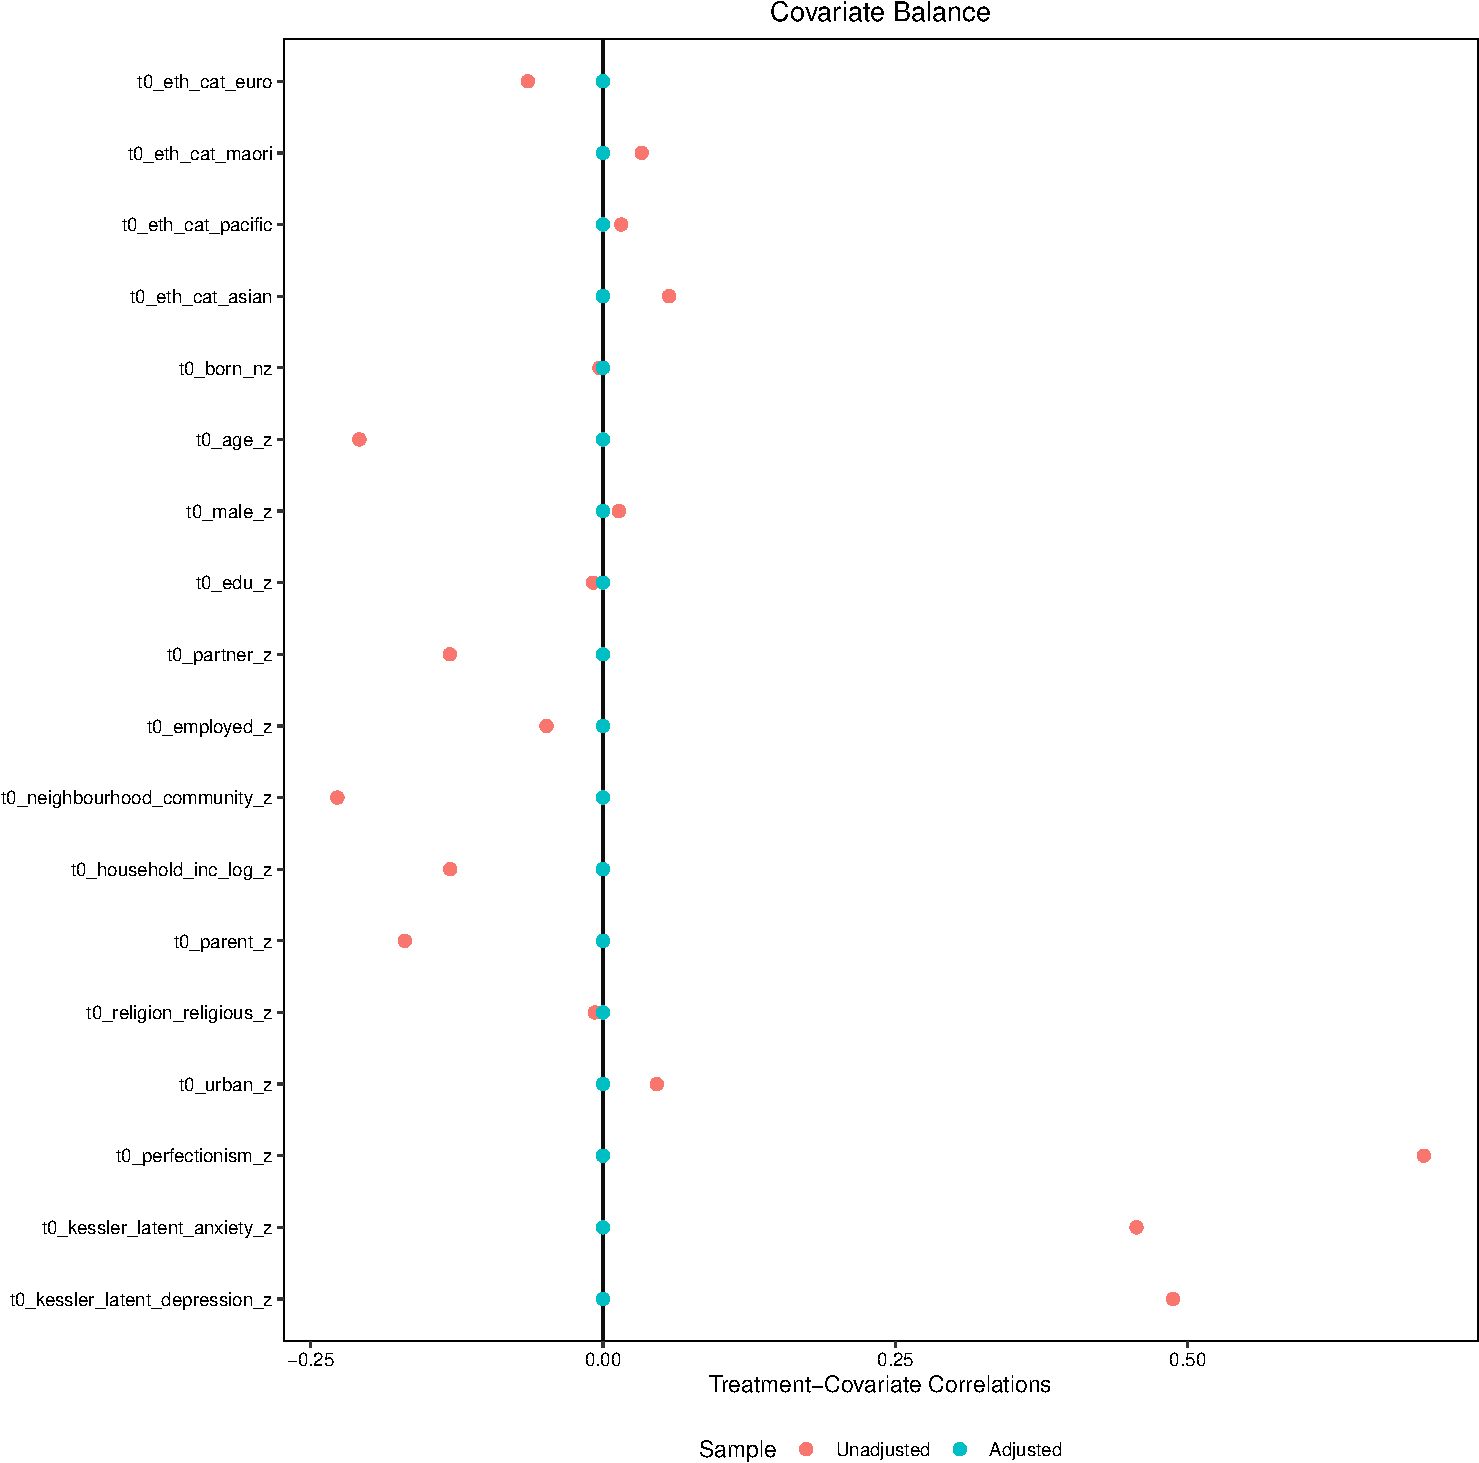
\includegraphics{example-manuscript_files/figure-pdf/fig-match_1-1.pdf}

}

\caption{\label{fig-match_1}This figure shows the imbalance in
covariates on the treatment}

\end{figure}%

\subsection{Appendix D: Baseline and End of Study Outcome
Statistics}\label{appendix-outcomes}

\begin{longtable}[]{@{}
  >{\raggedright\arraybackslash}p{(\columnwidth - 4\tabcolsep) * \real{0.4167}}
  >{\raggedright\arraybackslash}p{(\columnwidth - 4\tabcolsep) * \real{0.2917}}
  >{\raggedright\arraybackslash}p{(\columnwidth - 4\tabcolsep) * \real{0.2917}}@{}}

\caption{\label{tbl-table-outcomes}Outcomes at baseline and
end-of-study}

\tabularnewline

\toprule\noalign{}
\begin{minipage}[b]{\linewidth}\raggedright
\textbf{Outcome Variables by Wave}
\end{minipage} & \begin{minipage}[b]{\linewidth}\raggedright
\textbf{2018}, N = 19,997
\end{minipage} & \begin{minipage}[b]{\linewidth}\raggedright
\textbf{2020}, N = 19,997
\end{minipage} \\
\midrule\noalign{}
\endhead
\bottomrule\noalign{}
\endlastfoot
\textbf{Kessler Latent Anxiety} & 1.04 (0.66, 1.68) & 1.03 (0.65,
1.67) \\
Unknown & 203 & 6,768 \\
\textbf{Kessler Latent Depression} & 0.33 (0.01, 0.98) & 0.32 (0.01,
0.97) \\
Unknown & 207 & 6,765 \\

\end{longtable}

Table~\ref{tbl-table-outcomes} presents baseline and end-of-study
descriptive statistics for the outcome variables.

\newpage{}

\subsection*{References}\label{references}
\addcontentsline{toc}{subsection}{References}

\phantomsection\label{refs}
\begin{CSLReferences}{1}{0}
\bibitem[\citeproctext]{ref-atkinson2019}
Atkinson, J, Salmond, C, and Crampton, P (2019) \emph{NZDep2018 index of
deprivation, user{'}s manual.}, Wellington.

\bibitem[\citeproctext]{ref-bulbulia2024PRACTICAL}
Bulbulia, J (2024a) A practical guide to causal inference in three-wave
panel studies. \emph{PsyArXiv Preprints}.
doi:\href{https://doi.org/10.31234/osf.io/uyg3d}{10.31234/osf.io/uyg3d}.

\bibitem[\citeproctext]{ref-margot2024}
Bulbulia, JA (2024b) \emph{Margot: MARGinal observational
treatment-effects}.
doi:\href{https://doi.org/10.5281/zenodo.10907724}{10.5281/zenodo.10907724}.

\bibitem[\citeproctext]{ref-bulbulia2023a}
Bulbulia, JA, Afzali, MU, Yogeeswaran, K, and Sibley, CG (2023)
Long-term causal effects of far-right terrorism in {N}ew {Z}ealand.
\emph{PNAS Nexus}, \textbf{2}(8), pgad242.

\bibitem[\citeproctext]{ref-Bulbulia_2015}
Bulbulia, JA, Shaver, JH, Greaves, L, Sosis, R, and Sibley, CG (2015)
Religion and parental cooperation: An empirical test of slone's sexual
signaling model. In S. J. D. amd Van Slyke J., ed., \emph{The attraction
of religion: A sexual selectionist account}, Bloomsbury Press, 29--62.

\bibitem[\citeproctext]{ref-campbell2004}
Campbell, WK, Bonacci, AM, Shelton, J, Exline, JJ, and Bushman, BJ
(2004) Psychological entitlement: Interpersonal consequences and
validation of a self-report measure. \emph{Journal of Personality
Assessment}, \textbf{83}(1), 29--45.

\bibitem[\citeproctext]{ref-chatton2020}
Chatton, A, Le Borgne, F, Leyrat, C, \ldots{} Foucher, Y (2020)
G-computation, propensity score-based methods, and targeted maximum
likelihood estimator for causal inference with different covariates
sets: a comparative simulation study. \emph{Scientific Reports},
\textbf{10}(1), 9219.
doi:\href{https://doi.org/10.1038/s41598-020-65917-x}{10.1038/s41598-020-65917-x}.

\bibitem[\citeproctext]{ref-xgboost2023}
Chen, T, He, T, Benesty, M, \ldots{} Yuan, J (2023) \emph{Xgboost:
Extreme gradient boosting}. Retrieved from
\url{https://CRAN.R-project.org/package=xgboost}

\bibitem[\citeproctext]{ref-danaei2012}
Danaei, G, Tavakkoli, M, and Hernán, MA (2012) Bias in observational
studies of prevalent users: lessons for comparative effectiveness
research from a meta-analysis of statins. \emph{American Journal of
Epidemiology}, \textbf{175}(4), 250--262.
doi:\href{https://doi.org/10.1093/aje/kwr301}{10.1093/aje/kwr301}.

\bibitem[\citeproctext]{ref-decoulanges1903}
De Coulanges, F (1903) \emph{La cité antique: Étude sur le culte, le
droit, les institutions de la grèce et de rome}, Hachette.

\bibitem[\citeproctext]{ref-duxedaz2021}
Díaz, I, Williams, N, Hoffman, KL, and Schenck, EJ (2021) Non-parametric
causal effects based on longitudinal modified treatment policies.
\emph{Journal of the American Statistical Association}.
doi:\href{https://doi.org/10.1080/01621459.2021.1955691}{10.1080/01621459.2021.1955691}.

\bibitem[\citeproctext]{ref-diaz2023lmtp}
Díaz, I, Williams, N, Hoffman, KL, and Schenck, EJ (2023) Nonparametric
causal effects based on longitudinal modified treatment policies.
\emph{Journal of the American Statistical Association},
\textbf{118}(542), 846--857.
doi:\href{https://doi.org/10.1080/01621459.2021.1955691}{10.1080/01621459.2021.1955691}.

\bibitem[\citeproctext]{ref-diaz2021nonparametric}
Dı́az, I, Hejazi, NS, Rudolph, KE, and Der Laan, MJ van (2021)
Nonparametric efficient causal mediation with intermediate confounders.
\emph{Biometrika}, \textbf{108}(3), 627--641.

\bibitem[\citeproctext]{ref-fahy2017}
Fahy, KM, Lee, A, and Milne, BJ (2017b) \emph{New Zealand socio-economic
index 2013}, Wellington, New Zealand: Statistics New Zealand-Tatauranga
Aotearoa.

\bibitem[\citeproctext]{ref-fahy2017a}
Fahy, KM, Lee, A, and Milne, BJ (2017a) \emph{New Zealand socio-economic
index 2013}, Wellington, New Zealand: Statistics New Zealand-Tatauranga
Aotearoa.

\bibitem[\citeproctext]{ref-fraser_coding_2020}
Fraser, G, Bulbulia, J, Greaves, LM, Wilson, MS, and Sibley, CG (2020)
Coding responses to an open-ended gender measure in a {N}ew {Z}ealand
national sample. \emph{The Journal of Sex Research}, \textbf{57}(8),
979--986.
doi:\href{https://doi.org/10.1080/00224499.2019.1687640}{10.1080/00224499.2019.1687640}.

\bibitem[\citeproctext]{ref-haneuse2013estimation}
Haneuse, S, and Rotnitzky, A (2013) Estimation of the effect of
interventions that modify the received treatment. \emph{Statistics in
Medicine}, \textbf{32}(30), 5260--5277.

\bibitem[\citeproctext]{ref-hernan2024WHATIF}
Hernan, MA, and Robins, JM (2024) \emph{Causal inference: What if?},
Taylor \& Francis. Retrieved from
\url{https://www.hsph.harvard.edu/miguel-hernan/causal-inference-book/}

\bibitem[\citeproctext]{ref-hernan2024stating}
Hernán, MA, and Greenland, S (2024) Why stating hypotheses in grant
applications is unnecessary. \emph{JAMA}, \textbf{331}(4), 285--286.

\bibitem[\citeproctext]{ref-hoffman2023}
Hoffman, KL, Salazar-Barreto, D, Rudolph, KE, and Díaz, I (2023)
Introducing longitudinal modified treatment policies: A unified
framework for studying complex exposures.
doi:\href{https://doi.org/10.48550/arXiv.2304.09460}{10.48550/arXiv.2304.09460}.

\bibitem[\citeproctext]{ref-hoffman2022}
Hoffman, KL, Schenck, EJ, Satlin, MJ, \ldots{} Díaz, I (2022) Comparison
of a target trial emulation framework vs cox regression to estimate the
association of corticosteroids with COVID-19 mortality. \emph{JAMA
Network Open}, \textbf{5}(10), e2234425.
doi:\href{https://doi.org/10.1001/jamanetworkopen.2022.34425}{10.1001/jamanetworkopen.2022.34425}.

\bibitem[\citeproctext]{ref-hoverd_religious_2010}
Hoverd, WJ, and Sibley, CG (2010) Religious and denominational diversity
in new zealand 2009. \emph{New Zealand Sociology}, \textbf{25}(2),
59--87.

\bibitem[\citeproctext]{ref-johnson2005}
Johnson, DD (2005) God{'}s punishment and public goods: A test of the
supernatural punishment hypothesis in 186 world cultures. \emph{Human
Nature}, \textbf{16}, 410--446.

\bibitem[\citeproctext]{ref-jost_end_2006-1}
Jost, JT (2006) The end of the end of ideology. \emph{American
Psychologist}, \textbf{61}(7), 651--670.
doi:\href{https://doi.org/10.1037/0003-066X.61.7.651}{10.1037/0003-066X.61.7.651}.

\bibitem[\citeproctext]{ref-van2012targeted}
Laan, MJ van der, and Gruber, S (2012) Targeted minimum loss based
estimation of causal effects of multiple time point interventions.
\emph{The International Journal of Biostatistics}, \textbf{8}(1).

\bibitem[\citeproctext]{ref-van2014discussion}
Laan, MJ van der, Luedtke, AR, and Dı́az, I (2014) Discussion of
identification, estimation and approximation of risk under interventions
that depend on the natural value of treatment using observational data,
by {J}essica {Y}oung, {M}iguel {H}ern{á}n, and {J}ames {R}obins.
\emph{Epidemiologic Methods}, \textbf{3}(1), 21--31.

\bibitem[\citeproctext]{ref-linden2020EVALUE}
Linden, A, Mathur, MB, and VanderWeele, TJ (2020) Conducting sensitivity
analysis for unmeasured confounding in observational studies using
e-values: The evalue package. \emph{The Stata Journal}, \textbf{20}(1),
162--175.

\bibitem[\citeproctext]{ref-major2023exploring}
Major-Smith, D (2023) Exploring causality from observational data: An
example assessing whether religiosity promotes cooperation.
\emph{Evolutionary Human Sciences}, \textbf{5}, e22.

\bibitem[\citeproctext]{ref-diaz2012population}
Muñoz, ID, and Van Der Laan, M (2012) Population intervention causal
effects based on stochastic interventions. \emph{Biometrics},
\textbf{68}(2), 541--549.

\bibitem[\citeproctext]{ref-norenzayan2016}
Norenzayan, A, Shariff, AF, Gervais, WM, \ldots{} Henrich, J (2016) The
cultural evolution of prosocial religions. \emph{Behavioral and Brain
Sciences}, \textbf{39}, e1.
doi:\href{https://doi.org/10.1017/S0140525X14001356}{10.1017/S0140525X14001356}.

\bibitem[\citeproctext]{ref-pearl2009}
Pearl, J (2009) \emph{\href{https://doi.org/10.1214/09-SS057}{Causal
inference in statistics: An overview}}.

\bibitem[\citeproctext]{ref-polley2023}
Polley, E, LeDell, E, Kennedy, C, and Laan, M van der (2023)
\emph{SuperLearner: Super learner prediction}. Retrieved from
\url{https://CRAN.R-project.org/package=SuperLearner}

\bibitem[\citeproctext]{ref-richardson2023nested}
Richardson, TS, Evans, RJ, Robins, JM, and Shpitser, I (2023) Nested
{M}arkov properties for acyclic directed mixed graphs. \emph{The Annals
of Statistics}, \textbf{51}(1), 334--361.

\bibitem[\citeproctext]{ref-richardson2013swigsprimer}
Richardson, TS, and Robins, JM (2013) Single world intervention graphs:
A primer. In \emph{Second UAI workshop on causal structure learning,
{B}ellevue, {W}ashington}, Citeseer. Retrieved from
\url{https://citeseerx.ist.psu.edu/document?repid=rep1&type=pdf&doi=07bbcb458109d2663acc0d098e8913892389a2a7}

\bibitem[\citeproctext]{ref-richardson2023potential}
Richardson, TS, and Robins, JM (2023) Potential outcome and decision
theoretic foundations for statistical causality. \emph{Journal of Causal
Inference}, \textbf{11}(1), 20220012.

\bibitem[\citeproctext]{ref-robins1986}
Robins, J (1986) A new approach to causal inference in mortality studies
with a sustained exposure period---application to control of the healthy
worker survivor effect. \emph{Mathematical Modelling}, \textbf{7}(9-12),
1393--1512.

\bibitem[\citeproctext]{ref-robins2010alternative}
Robins, JM, and Richardson, TS (2010) Alternative graphical causal
models and the identification of direct effects. \emph{Causality and
Psychopathology: Finding the Determinants of Disorders and Their Cures},
\textbf{84}, 103--158.

\bibitem[\citeproctext]{ref-rubin2005}
Rubin, DB (2005) Causal inference using potential outcomes: Design,
modeling, decisions. \emph{Journal of the American Statistical
Association}, \textbf{100}(469), 322--331. Retrieved from
\url{https://www.jstor.org/stable/27590541}

\bibitem[\citeproctext]{ref-schloss2011evolutionary}
Schloss, JP, and Murray, MJ (2011) Evolutionary accounts of belief in
supernatural punishment: A critical review. \emph{Religion, Brain \&
Behavior}, \textbf{1}(1), 46--99.

\bibitem[\citeproctext]{ref-shiba2021using}
Shiba, K, and Kawahara, T (2021) Using propensity scores for causal
inference: Pitfalls and tips. \emph{Journal of Epidemiology},
\textbf{31}(8), 457--463.

\bibitem[\citeproctext]{ref-shpitser2022multivariate}
Shpitser, I, Richardson, TS, and Robins, JM (2022) Multivariate
counterfactual systems and causal graphical models. In
\emph{Probabilistic and causal inference: The works of {J}udea {P}earl},
813--852.

\bibitem[\citeproctext]{ref-shpitser2016causal}
Shpitser, I, and Tchetgen, ET (2016) Causal inference with a graphical
hierarchy of interventions. \emph{Annals of Statistics}, \textbf{44}(6),
2433.

\bibitem[\citeproctext]{ref-sibley2012}
Sibley, C. G., and Bulbulia, JA (2012) Healing those who need healing:
How religious practice affects social belonging. \emph{Journal for the
Cognitive Science of Religion}, \textbf{1}, 29--45.

\bibitem[\citeproctext]{ref-sibley2021}
Sibley, CG (2021)
\emph{\href{https://doi.org/10.31234/osf.io/wgqvy}{Sampling procedure
and sample details for the new zealand attitudes and values study}}.

\bibitem[\citeproctext]{ref-sibley2011}
Sibley, CG, Luyten, N, Purnomo, M, \ldots{} Robertson, A (2011) The
Mini-IPIP6: Validation and extension of a short measure of the Big-Six
factors of personality in New Zealand. \emph{New Zealand Journal of
Psychology}, \textbf{40}(3), 142--159.

\bibitem[\citeproctext]{ref-sosis2003cooperation}
Sosis, R, and Bressler, ER (2003) Cooperation and commune longevity: A
test of the costly signaling theory of religion. \emph{Cross-Cultural
Research}, \textbf{37}(2), 211--239.

\bibitem[\citeproctext]{ref-neyman1923}
Splawa-Neyman, J, Dabrowska, DM, and Speed, TP (1990) On the application
of probability theory to agricultural experiments. Essay on principles.
Section 9. \emph{Statistical Science}, 465--472.

\bibitem[\citeproctext]{ref-swanson1967}
Swanson, GE (1967) Religion and regime: A sociological account of the
{R}eformation.

\bibitem[\citeproctext]{ref-vanbuuren2018}
Van Buuren, S (2018) \emph{Flexible imputation of missing data}, CRC
press.

\bibitem[\citeproctext]{ref-van2014targeted}
Van der Laan, MJ (2014) Targeted estimation of nuisance parameters to
obtain valid statistical inference. \emph{The International Journal of
Biostatistics}, \textbf{10}(1), 29--57.

\bibitem[\citeproctext]{ref-vanderlaan2011}
Van Der Laan, MJ, and Rose, S (2011) \emph{Targeted Learning: Causal
Inference for Observational and Experimental Data}, New York, NY:
Springer. Retrieved from
\url{https://link.springer.com/10.1007/978-1-4419-9782-1}

\bibitem[\citeproctext]{ref-vanderlaan2018}
Van Der Laan, MJ, and Rose, S (2018) \emph{Targeted Learning in Data
Science: Causal Inference for Complex Longitudinal Studies}, Cham:
Springer International Publishing. Retrieved from
\url{http://link.springer.com/10.1007/978-3-319-65304-4}

\bibitem[\citeproctext]{ref-vanderweele2009}
VanderWeele, TJ (2009) Concerning the consistency assumption in causal
inference. \emph{Epidemiology}, \textbf{20}(6), 880.
doi:\href{https://doi.org/10.1097/EDE.0b013e3181bd5638}{10.1097/EDE.0b013e3181bd5638}.

\bibitem[\citeproctext]{ref-vanderweele2017causaleffectsService}
VanderWeele, TJ (2017) Causal effects of religious service attendance?
\emph{Social Psychiatry and Psychiatric Epidemiology}, \textbf{52},
1331--1336.

\bibitem[\citeproctext]{ref-vanderweele2019}
VanderWeele, TJ (2019) Principles of confounder selection.
\emph{European Journal of Epidemiology}, \textbf{34}(3), 211--219.

\bibitem[\citeproctext]{ref-vanderweele2021can}
VanderWeele, TJ (2021) Can sophisticated study designs with regression
analyses of observational data provide causal inferences? \emph{JAMA
Psychiatry}, \textbf{78}(3), 244--246.

\bibitem[\citeproctext]{ref-vanderweele2017}
VanderWeele, TJ, and Ding, P (2017) Sensitivity analysis in
observational research: Introducing the e-value. \emph{Annals of
Internal Medicine}, \textbf{167}(4), 268--274.
doi:\href{https://doi.org/10.7326/M16-2607}{10.7326/M16-2607}.

\bibitem[\citeproctext]{ref-vanderweele2013}
VanderWeele, TJ, and Hernan, MA (2013) Causal inference under multiple
versions of treatment. \emph{Journal of Causal Inference},
\textbf{1}(1), 1--20.

\bibitem[\citeproctext]{ref-vanderweele2012MEASUREMENT}
VanderWeele, TJ, and Hernán, MA (2012) Results on differential and
dependent measurement error of the exposure and the outcome using signed
directed acyclic graphs. \emph{American Journal of Epidemiology},
\textbf{175}(12), 1303--1310.
doi:\href{https://doi.org/10.1093/aje/kwr458}{10.1093/aje/kwr458}.

\bibitem[\citeproctext]{ref-vanderweele2020}
VanderWeele, TJ, Mathur, MB, and Chen, Y (2020) Outcome-wide
longitudinal designs for causal inference: A new template for empirical
studies. \emph{Statistical Science}, \textbf{35}(3), 437--466.

\bibitem[\citeproctext]{ref-verbrugge1997}
Verbrugge, LM (1997) A global disability indicator. \emph{Journal of
Aging Studies}, \textbf{11}(4), 337--362.
doi:\href{https://doi.org/10.1016/S0890-4065(97)90026-8}{10.1016/S0890-4065(97)90026-8}.

\bibitem[\citeproctext]{ref-watts2016}
Watts, J, Bulbulia, J. A., Gray, RD, and Atkinson, QD (2016) Clarity and
causality needed in claims about big gods., \textbf{39}, 41--42.
doi:\href{https://doi.org/DOI:10.1017/S0140525X15000576}{DOI:10.1017/S0140525X15000576}.

\bibitem[\citeproctext]{ref-watts2015}
Watts, J, Greenhill, SJ, Atkinson, QD, Currie, TE, Bulbulia, J, and
Gray, RD (2015) \emph{Broad supernatural punishment but not moralizing
high gods precede the evolution of political complexity in
{A}ustronesia} \emph{Proceedings of the Royal Society B: Biological
Sciences}, Vol. 282, The Royal Society, 20142556.

\bibitem[\citeproctext]{ref-westreich2010}
Westreich, D, and Cole, SR (2010) Invited commentary: positivity in
practice. \emph{American Journal of Epidemiology}, \textbf{171}(6).
doi:\href{https://doi.org/10.1093/aje/kwp436}{10.1093/aje/kwp436}.

\bibitem[\citeproctext]{ref-wheatley1971}
Wheatley, P (1971) \emph{The pivot of the four quarters : A preliminary
enquiry into the origins and character of the ancient chinese city},
Edinburgh University Press. Retrieved from
\url{https://cir.nii.ac.jp/crid/1130000795717727104}

\bibitem[\citeproctext]{ref-whitehouse2023}
Whitehouse, H, Francois, P, Savage, PE, \ldots{} Turchin, P (2023)
Testing the big gods hypothesis with global historical data: A review
and retake. \emph{Religion, Brain \& Behavior}, \textbf{13}(2),
124--166.

\bibitem[\citeproctext]{ref-williams2021}
Williams, NT, and Díaz, I (2021) \emph{{l}mtp: Non-parametric causal
effects of feasible interventions based on modified treatment policies}.
doi:\href{https://doi.org/10.5281/zenodo.3874931}{10.5281/zenodo.3874931}.

\bibitem[\citeproctext]{ref-Ranger2017}
Wright, MN, and Ziegler, A (2017) {ranger}: A fast implementation of
random forests for high dimensional data in {C++} and {R}. \emph{Journal
of Statistical Software}, \textbf{77}(1), 1--17.
doi:\href{https://doi.org/10.18637/jss.v077.i01}{10.18637/jss.v077.i01}.

\bibitem[\citeproctext]{ref-young2014identification}
Young, JG, Hernán, MA, and Robins, JM (2014) Identification, estimation
and approximation of risk under interventions that depend on the natural
value of treatment using observational data. \emph{Epidemiologic
Methods}, \textbf{3}(1), 1--19.

\bibitem[\citeproctext]{ref-zhang2023shouldMultipleImputation}
Zhang, J, Dashti, SG, Carlin, JB, Lee, KJ, and Moreno-Betancur, M (2023)
Should multiple imputation be stratified by exposure group when
estimating causal effects via outcome regression in observational
studies? \emph{BMC Medical Research Methodology}, \textbf{23}(1), 42.

\end{CSLReferences}



\end{document}
